\documentclass[letterpaper, conference]{IEEEtran}

\usepackage{amsmath}
\usepackage{mathabx}
\DeclareMathOperator*{\argmax}{argmax}

\usepackage{pgfplots}
\pgfplotsset{compat=1.5.1}

\usetikzlibrary{matrix}

%\usepackage{titlesec}
%\titlespacing*{\subsection}{0pt}{1.1\baselineskip}{\baselineskip}
%\setlength{\parindent}{2em}
\setlength{\parskip}{0.7em}

\usepackage{url}

\begin{document}

\title{A Discrete Bayesian Classifier \\
  \large Machine Learning Midterm Report}

\author{
  \IEEEauthorblockN{Alvaro Faundez}
  \IEEEauthorblockA{
    \textit{Master in Data Science's Program, first year}\\
    \textit{CUNY Graduate Center}\\
    \textit{alvaro@faundez.net}
  }
}

\maketitle

\begin{abstract}

This report details the implementation of a discrete Bayesian classifier. The classifier requirements are a dataset and an economic gain matrix for input. The process calculates the class, measurement conditional, and class conditional probabilities from the dataset, all needed for the Bayes theorem. It outputs the Bayes rule, the confusion matrix, and the expected gain matrix associated with the input used. After completing the training and predicting steps, small perturbations are introduced in the measurement conditional probabilities of every misclassification, obtaining an improvement, as expected, in the expected gain (after recalculating all the classifier's outputs). The experiments included using the dataset split into equally sized training and test sets and using K-fold cross-validation. The dataset was created using synthetic probabilities distribution. A series of results are detailed in the appendix.

\end{abstract}

\section{Introduction}


The discrete Bayesian classifier is a popular predictive classifier broadly used in Machine Learning, based on the Bayes Theorem [\ref{eq:bayes-theorem}].

\begin{equation}\label{eq:bayes-theorem}
  P(A \mid B) = \frac{P(B \mid A)\mathbin{}P(A)}{P(B)}
\end{equation}

A discrete Bayesian classifier, given a set of classifications, a measurement space, and a dataset, uses the Bayes theorem to compute the conditional probabilities and the Bayes rule decision needed to perform classification. It can be optimized using an Economic Gain matrix, by maximizing the Expected Gain obtained using the Bayes decision rule.

In our case, given a set $C$ of $K$ discrete classifications [\ref{eq:classes-set}] and a discrete measurement space $D$, result of the cartesian product of $N$ discrete measurements $L_n$ [\ref{eq:measurement-space}], the classifier is a function assigning a unique classification $c \in C$ to any measurement $\vec{d} \in D$.

\begin{equation}\label{eq:classes-set}
C = \{\,c_1,\, \dots,\, c_{K}\,\}
\end{equation}


\begin{gather}\label{eq:measurement-space}
D = \bigtimes_{n=1}^{N} L_n \\
L_n = \{l_{n_1},\, \dots,\, l_{n_{M_n}}\},\, \forall n \in { 1, ..., N }, M_n = \vert L_n\vert
\end{gather}

For the classification, the following inputs are required:

\begin{itemize}
  \item the discrete classification cardinality, $K$
  \item the cardinalities of each discrete measurement, $\vert L_n \vert,\, n \in N$
  \item an Economic Gain Matrix, $e^{K \times K}$
  \item a dataset with $Z$ measurements with matching $Z$ classifications. 
\end{itemize}

The Economic Gain matrix, $e$, is a $K \times K$ matrix that defines the gain (or cost) of making the right (or wrong) classifications [\ref{eq:economic-gain-matrix}]. Each column will represent an assigned class, and each row will represent the true class. Then, every element $e(c_i,\, c_j) \in e$ represent the gain or cost of assigning the class $c_j$ when the true class was $c_i$. The economic gain usually is positive for every correct classification and non-positive for every other case. The identity matrix is an example of an economic gain matrix.

\begin{equation}\label{eq:economic-gain-matrix}
  e^{K \times K} = \begin{pmatrix}
    e(c_1,c_1) & \cdots & e(c_1,c_K) \\
      \vdots   & \ddots &    \vdots   \\
    e(c_K,c_1) & \cdots & e(c_K,c_K)
  \end{pmatrix}
\end{equation}


The economical consequences of the classifier are determined by the Expected Gain Matrix $G^{K \times K}$. Each element $g$ is the multiplication between the economic gain $e(i,\, j) \in K$ and the probability of the true class $c_i$ being assigned class $c_j$, $P(c_i,\, c_j)$ [\ref{eq:expected-gain-matrix}].

\begin{equation}\label{eq:expected-gain-matrix}
  G^{K \times K} = \begin{pmatrix}
    e(c_1,c_1)P(c_1,c_1) & \cdots & e(c_1,c_K)P(c_1,c_K) \\
                \vdots   & \ddots &    \vdots   \\
    e(c_K,c_1)P(c_K,c_1) & \cdots & e(c_K,c_K)P(c_K,c_K)
  \end{pmatrix}
\end{equation}

The Expected Gain of the classifier is the sum of all the elements of the Expected Gain Matrix [\ref{eq:expected-gain}].

\begin{equation}\label{eq:expected-gain}
  E[e] = \sum_{i \in K} \sum_{j \in K}e(c_i,\,c_k)\mathbin{}P(c_i,\,c_k)
\end{equation}

The goal is to determine the Bayes decision rule that maximizes the Expected Gain of the classifier, $E$.

A critical step in the construction of the classifier is the building of the Bayes decision rule $f_{\vec{d}}$ [\ref{eq:bayes-rule}]. The Bayes decision rule will assign 1 to the class that maximizes the Expected Gain [\ref{eq:bayes-argmax}], and 0 otherwise.

\begin{equation}\label{eq:bayes-rule}
  f_d(c_j) =
  \begin{cases}
  1 & j = k \\
  0 & j \neq k
  \end{cases}
\end{equation}

\begin{equation}\label{eq:bayes-argmax}
  \argmax_{c_k \in C} \sum_{j = 1}^{K} e(c_j, c_k)\mathbin{}P(c_j, \vec{d})
\end{equation}

The Expected Gain can be written in function of the Bayes decision rule [\label{eq:bayes-expected-gain}].

\begin{equation}\label{eq:bayes-expected-gain}
  E[e, f] = \sum_{i \in K} \sum_{j \in K}\sum_{\vec{d} \in D}f_{\vec{d}}(c_j)\mathbin{}e(c_i,\, c_j)\mathbin{}P(c_i,\,\vec{d})
\end{equation}

To obtain $f_{\vec{d}}$ and $P(c,\, \vec{d})$, it is necessary to calculate the posterior probability of assigning a class $c$ to measurement $\vec{d}$, $P(c \mid \vec{d})$, using the prior class probability $P(c)$ and the probability of the measurement given the class $P(\vec{d} \mid c)$ [\ref{eq:bayes-theorem-proportional}].

\begin{equation} \label{eq:bayes-theorem-proportional}
  P(c,\, \vec{d}) \mathbin{\propto} P(\vec{d} \mid c) \mathbin{} P(c)
\end{equation}

This report details an implementation of a discrete Bayesian classifier used to implement the classifier. A technical overview explains the design and implementation, along with the results of the experiments executed.

The definition and implementation include:

\begin{itemize}
  \item Classification and measurement dimensions, including pseudo-random probabilities and cumulative distribution functions
  \item Space definition and linear addresses
  \item Class prior and conditional probabilities
  \item Classifier optimization using an economic gain matrix
  \item Dataset definition and generation of pseudo-random synthetic data
  \item Experimentation framework with two types of cross-validation
\end{itemize}

The classifier's performance is tested by adding small perturbations to the class conditional, increasing the expected gain. The increase was tested using are training/test and k-folds cross-validation.

\section{Technical}

\subsection{Definitions}

In order to explain the implementation, a few concepts must be discussed.

\subsubsection{Dimension}
A dimension is a 1-dimensional set of $M$ correlatives integer numbers from 1 to $K$. Any 1-dimensional $L$ set has a Probability Mass Function $P$ and a Cumulative Distribution Function $Q$ [\ref{fig:pmf-cdf}]. The $P$ set will be created by generating a set $R$ with $K$ pseudo-random numbers $r_1, ...r_K$ scaled to 1 $p_1, ...r_K$ [\ref{eq:pmf}]. The $Q$ set is sequence of cumulative sum of the probabilities in the $P$ [\ref{eq:cdf}].

\pgfplotstableread[row sep=\\,col sep=&]{
value & Probability \\
1 & 0.07155134805450836 \\
2 & 0.12997048848822798 \\
3 & 0.1386944981818227 \\
4 & 0.04197817941692496 \\
5 & 0.16869281585900325 \\
6 & 0.16136757309412517 \\
7 & 0.03288486428939286 \\
8 & 0.1571494317575896 \\
9 & 0.07917145577927193 \\
10 & 0.0185393450791332 \\
}\pmf

\pgfplotstableread[row sep=\\,col sep=&]{
value & Cumulative Probability \\
1 & 0.07155134805450836 \\
2 & 0.20152183654273634 \\
3 & 0.34021633472455903 \\
4 & 0.382194514141484 \\
5 & 0.5508873300004873 \\
6 & 0.7122549030946125 \\
7 & 0.7451397673840053 \\
8 & 0.9022891991415949 \\
9 & 0.9814606549208669 \\
10 & 1.0 \\
}\cdf

\begin{figure}
  \begin{tikzpicture}
    \begin{axis}[
      ybar,
      x label style={at={(axis description cs:0.5,-0.1)}, anchor=north},
      xlabel={Dimension values},
      legend pos=north west
      ]
      \addplot table[x=value,y=Probability]{\pmf};
      \addplot table[x=value,y=Cumulative Probability]{\cdf};
      \addlegendentry{PMF}
      \addlegendentry{CDF}
    \end{axis}
  \end{tikzpicture}
  \caption{PMF and CDF values for a dimension with 10 possible values}
\end{figure}

\begin{equation}\label{eq:pmf}
  \begin{aligned}
  R &= \{r_1, \dots, r_K\} \\
  P &= \Bigl\{p_i \mid p_i = \frac{r_i}{r_{\sum_{i = 1}^{K} r_i}}, r_i \in R \Bigr\}
  \end{aligned}
\end{equation}

\begin{equation}\label{eq:cdf}
Q = \Bigl\{q_i \mid q_i = \sum_{j = 1}^{K} p_j, p_j \in P \Bigr\}
\end{equation}

The classifications set $C$ and every measurement $L_n$ are 1-dimensional set with their corresponding probabilities sets.

The cumulative distribution functions will be used to generate pseudo-random numbers in the 1-dimensional space: Given a cumulative distribution function $Q$ belonging to the dimension $M$, $f_Q$ will take a number $r \in [0, 1]$. $f_Q$ and assign it the number $k \in M$ according to the relative position of $r$ compared with the numbers in $Q$ [\ref{eq:cumulative}].

\begin{equation}\label{eq:cumulative}
  f_Q(r) =
  \begin{cases}
  1 & r < q_1 \\
  k & q_{k - 1} < r \leq q_k,\, k \in M - \{1\} \\
  \end{cases}
\end{equation}

\subsubsection{Measurement Space}
The measurement space $D$ is the cartesian product of a set of measurements \label{eq:measurement-space}. Every element in $\vec{d} \in D$ is a vector where every value corresponds to a measurement value [\ref{eq:measurements-vector}].

\begin{equation}\label{eq:measurements-vector}
  \vec{d} = (d_0, ..., d_N), \vec{d}_i \in L_n
\end{equation}

\subsubsection{Linear Space}
Each element in the measurement space can be mapped to a linear space using a bijective function $f_D$ that take a vector and transform it to an integer value $l \in \mathcal{L}$ [\ref{eq:linear-address}].

\begin{equation}\label{eq:linear-address}
  \begin{aligned}
  \mathcal{L} &=& \{1, \dots, \prod_{i \in N} \mid L_i \mid\} \\
  f_D&:& \bigtimes_{n=1}^{N} L_n \longleftrightarrow \mathcal{L} \\
  \end{aligned}
\end{equation}

We will assume every dimension in the measurement space is independent between each other, allowing us to compute the probability of every element in the measurement space $P(\vec{d})$ as the multiplication of the probabilities of each measurement value in $\vec{d}$ [\ref{eq:prod:measurements}].

\begin{equation}\label{eq:prod:measurements}
  P(\vec{d}) = \prod_{i = 1}^{N} P(d_o), d_i \in L_n
\end{equation}

\subsubsection{Classifier}
The classifier is the element that assign a classification to a measurement. The classifier is initialized in the context of a classifications set and a measurement space.

\subsubsection{Dataset}
A sample dataset is formed by two sets of equal size $Z$: the data $ X = \{x_i \in D \mid i \in [1, Z]\}$ and the target $Y = \{ y_i \in C \mid i \in [1, Z]\}$.

\subsubsection{Experiment}
A experiment will be defined as the isolated instance that takes inputs and produce results. The experiments will defined dimensions, classifications, measurement space, classifier, and datasets.

During an experiment, immutable measurement space and classifications will be used during the whole process. This means that during the experiments, the cumulative probabilities distribution remain unchanged. The experiments will yield a classifier that will work over the measurement space and classifications in the experiment.

\subsubsection{Iteration}
An iteration within an experiment will enclose the using and modification of the classifier available. Each iteration in a sequence of iterations will include the changes made to the classifier by the previous iteration.

\subsubsection{Validation}
Two different validations are considered in an iteration:
\begin{itemize}
  \item Test-Validation sets: The sample dataset will be shuffled and divided in equal sized subsets. The test subset is meant to be used during an iteration; the validation set is meant to be used only at the end of an iteration [\ref{eq:test-validation}].
  \item V-fold sets: The sample dataset will be shuffled and divided into $V$ equal sized folds. A V round-robin iterations will select a different fold as validation set and i will join the resting folds as a testing set [\ref{eq:v-fold}].
  \item 
\end{itemize}

\begin{figure}\label{eq:test-validation}
  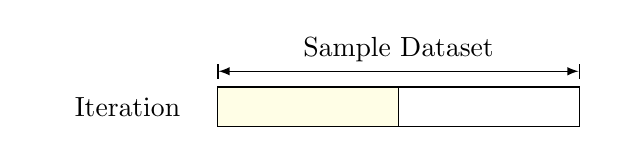
\begin{tikzpicture}
    \matrix (M) [matrix of nodes,
        nodes={minimum height = 5mm, minimum width = 2.3cm, outer sep=0, anchor=center, draw},
        column 1/.style={nodes={draw=none}, minimum width = 2.3cm},
        row sep=1mm, column sep=-\pgflinewidth, nodes in empty cells,
        e/.style={fill=yellow!10}
      ]
      {
        Iteration & |[e]| & \\
      };
    \draw (M-1-2.north west) ++(0,2mm) coordinate (LT) edge[|<->|, >= latex] node[above]{Sample Dataset} (LT-|M-1-3.north east);
  \end{tikzpicture}
  \caption{Test-Validation cross-validation.}
\end{figure}

\begin{figure}\label{eq:v-fold}
  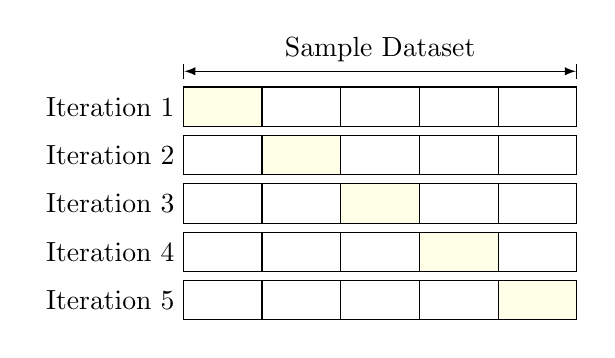
\begin{tikzpicture}
    \matrix (M) [matrix of nodes,
        nodes={minimum height = 5mm, minimum width = 1cm, outer sep=0, anchor=center, draw},
        column 1/.style={nodes={draw=none}, minimum width = 1cm},
        row sep=1mm, column sep=-\pgflinewidth, nodes in empty cells,
        e/.style={fill=yellow!10}
      ]
      {
        Iteration 1 & |[e]| & & & & \\
        Iteration 2 & & |[e]| & & & \\
        Iteration 3 & & & |[e]| & & \\
        Iteration 4 & & & & |[e]| & \\
        Iteration 5 & & & & & |[e]| \\
      };
    \draw (M-1-2.north west) ++(0,2mm) coordinate (LT) edge[|<->|, >= latex] node[above]{Sample Dataset} (LT-|M-1-6.north east);
  \end{tikzpicture}
  \caption{5-fold cross-validation. Each iteration uses the yellow fold as validation set and the rest folds as test set.}
\end{figure}
  

\subsection{Discrete Bayesian Classifier}

A classifier will assign a classification $c \in C$ to any measurement $\vec{d} \in D$ from the measurement space. Within the classifier, all measurement will be translated to the corresponding linear address. The following parameters will be set:

\begin{itemize}
  \item The list of $S$ linear addresses $l(\vec{d})$ for each $\vec{d} \in D$ [\ref{eq:linear-address}], stored in a $S$ sized vector
  \item Measurement probability $P(\vec{d})$ for each  $\vec{d} \in D$ [\ref{eq:prod:measurements}], stored in a $S$ sized vector
  \item Class probability $P(c)$ for each  $c \in C$ [\ref{eq:pmf}], stored in a $K$ sized vector
  \item Class conditional probabilities $P(\vec{d} \mid c)$. Each class $c \in C$ is assigned a probability mass distribution with $S$ probabilities [\ref{eq:pmf}], stored in a $K \times S$ matrix
\end{itemize}

After initializing the classifier, given an Economic Gain Matrix [\ref{eq:economic-gain-matrix}], the classifier can compute the elements needed to classify a measurement:

\begin{itemize}
  \item $P(c \mid \vec{d})$, the probabilities of class given a measurement, stored in an $S \times K$ matrix [\ref{eq:bayes-theorem}]
  \item $P(c,\, \vec{d})$ the probabilities of a class and a measurement, stored in an $S \times K$ matrix [\ref{eq:bayes-theorem-proportional}]
  \item the Bayes decision rule that optimize the expected gain for the Economic Gain Matrix, stored in an $S \times K$ matrix [\ref{eq:bayes-rule}]
  \item The Confusion Matrix, stored in an $K \times K$ matrix
  \item The Expected Gain Matrix, stored in an $K \times K$ matrix [\ref{eq:expected-gain-matrix}]
  \item The Expected Gain, the trace of the Expected Gain Matrix
\end{itemize}

This will produce a discrete Bayesian classifier optimized to get the maximum Expected Gain given a Economic Gain Matrix.

\section{Experiment}

To validate the discrete Bayesian classifier, a series of iteration will modify the probabilities of a measurement given a class $P(\vec{d} \mid c$ by adding small perturbations that must increase the Expected Gain monotonically to 1.

Each iteration in the experiment will compute an optimized classifier. Using that classifier dataset of $Z$ samples measurements and corresponding classifications, generating random measurements $\vec{d}$ and assign a random $c$ using as probability mass distribution $P(c \mid \vec{d})$. $Z$ will be define 10 times the classifications number times the measurement space [\ref{eq:sample-size}].

\begin{equation}\label{eq:sample-size}
  Z = 10 \times \mid C \mid \times \prod_{n \in N} |L_n|
\end{equation}

The classifier will be used to assign classification to each measurement in the test sample set:

\begin{itemize}
  \item For each assigned classification $c'$ made, if the classification is wrong a $\Delta$ perturbation will be added to $P(\vec{d} \mid c')$
  \item Normalize to 1 each column on the $P(\vec{d} \mid c)$ matrix
  \item Compute the classifier with the new probabilities
  \item Return the Expected Gain
\end{itemize}

The next iteration must do the exact same steps using the updated classifier.

\section{Experiment Results}











\subsection{Requirements}

To run the code, a Unix environment with Ruby 2.6+ is necessary. The code is available on GitHub at \url{https://github.com/afaundez/ml-midterm}.

To test the command and check the available options run:

\begin{verbatim}
  $ ./midterm --help
\end{verbatim}

\subsection{options}

For testing, the following parameters are available for configuration:

\begin{itemize}
    \item-s, --seed [INT]                 Pseudo-random seed, an integer. Default: nil
    \item-c, --classes [INT]              Class cardinality, an integer. Default 2
    \item-m, --measurements [INT]         Measurements size, an integer. Default 5
    \item    --measurement-min-cardinality [INT]
                                     Measurement Min Cardinality, an integer. Default 3
    \item    --measurement-max-cardinality [INT]
                                     Measurement Max Cardinality, an integer. Default 6
    \item    --sample-size [INT]          Sample size, an integer. Default to 10 times the  space addresses size.
    \item-i, --iterations [INT]           Iterations, an integer. Default 2
    \item-d, --delta [FLOAT]              Delta for conditionals improvement, a float. Default: 0.01
    \item    --no-overlap                 Generate classes based on measurements
    \item    --uniform                    Use uniform distribution on all dimensions
\end{itemize}

\subsection{Runtime}

\subsubsection{Build}

During the build, three significant abstractions are used: Dimension, Space, and DataSet.

The Dimension abstraction is meant to store the cardinality, probabilities distribution function, and cumulative distribution function of a single measurement or class. A dimension does not store values, but it can be used to generate random values using the distribution functions. A Dimension is defined by:

\begin{itemize}
  \item size
  \item pdf, generated based on the size
  \item cdf, generated based on the pdf
  \item distribution, whether to use a random or uniform distribution
\end{itemize}

The Space abstraction stores the single class dimension \ref{classes}, the collection of measurements dimensions \ref{dimensions}, and the class conditional probabilities. Since a space knows all the dimensions specifications, it is in charge of translating and measurement into a linear address and vice-versa. A space is defined by:

\begin{itemize}
\item class\_dimension, a Dimension instance
\item measurements\_dimensions, a collection of Dimension instances
\item likelihoods, random pdfs
\end{itemize}

The DataSet abstraction generates and stores measurement values and the associated classification, all bounded to a specific space. Since it has access to the data and space, it is in charge of the training and improving the class conditional probabilities, determining the Bayes Decision Rule, generating the Confusion Matrix, and calculating the Expected Gain. It is relevant that at the time of creating, the prior class probabilities are calculated and stored in the DataSet. A DataSet is defined by:

\begin{itemize}
\item size
\item space, a Space instance
\item samples, a collection of collections of measurements
\item class\_outcomes, counter of classes for prior class probabilities calculation
\item overlap, whether to assign classes with overlap
\end{itemize}

The Economic Gain Matrix is generated in this step. Even though it is a method, currently, the only matrix available is the identity matrix.

\subsubsection{Training}

Once a set of DataSet is created, the test DataSet is picked and left isolated, and the rest is used as train DataSet.

The training process consists of two steps. Using the training set and the economic gain matrix, the training outputs the Bayes decision rule and the expected gain. Then, using the Bayes decision rule, it generates the confusion matrix.


At the end of this process, the Space associated with the DataSet will store the measurement conditional probabilities $P(c \mid d)$ targeted in \ref{eq:bayes}.

\subsection{Optimization}

Now that the space is trained and the measurement conditional probabilities have been processed, using the delta as input, the dataset can improve the class conditional probabilities using the test DataSet. For each mismatched classification, the corresponding class conditional probability is incremented by the delta input, and the measurement probabilities are normalized to 1. This process yields an updated Space and accuracy obtained.

\section{Experimental Results}

Even though it is not a strict test, it is good to do a sanity check with a dummy case: one feature, one value measurement. It is expected to have an expected gain of 1.0 and an accuracy of 1.0.

Running

\begin{verbatim}
  bin/midterm --classes 1 --measurements 1
\end{verbatim}

yields, as expected,

\begin{verbatim}
Economic Gain Matrix
+---+
| 1 |
+---+

Train 0.
  Expected Gain: 1.0
  Confusion Matrix Trace: 1.0
  Accuracy: 1.0
Confusion Matrix
+-----+
| 1.0 |
+-----+

Test
  Expected Gain: 1.0
  Confusion Matrix Trace: 1.0
  Accuracy: 1.0
\end{verbatim}


The next step is to check the results using. Let us use two classes, five values measurements, and ten training sets, and start setting the seed number in order to have replicable experiments.

\subsection{First results}

\begin{verbatim}
  bin/midterm --classes 2 --measurements 5 \
    --iterations 10 --seed 1234
\end{verbatim}

The expected gain and accuracy do not seem to be correct

\begin{figure}[hbt]
  \label{fig:10-training-2-classes}
  \caption{}
\end{figure}

Incrementing the training iterations to 100 does not make real improvements; it keeps going up and down.

\begin{figure}[hbt]
  \label{fig:100-training-2-classes}
  \caption{}
\end{figure}

To identify the reason of these results, two options were added to the application, one to control the overlap in the class assignment to a measurement and how the probability distribution is generated.

\subsection{Probability distributions}

Since the method used to generate the probability distribution function for a dimension does not generate even probabilities for each value in the dimension, a parameter $--uniform$ was added to revert this and generate uniform distribution for the classes and measurement. The hypothesis was that by generating numbers evenly, the results would easier to understand.

Now, repeating the previous commands with the new parameter:

\begin{verbatim}
  bin/midterm --classes 2 --measurements 5 \
    --iterations 10 --seed 1234 \
    --uniform
\end{verbatim}

\begin{figure}[hbt]
  \label{fig:10-training-2-classes-uniform}
  \caption{}
\end{figure}

The expected gain does not seem to be improving, but the accuracy is set around $0.5$. It could be a sign that accuracy is bouncing between that particular number because now each class has the same probability of being assign to a measurement. Using 100 training iterations, the result is similar.

\begin{figure}[hbt]
  \label{fig:100-training-2-classes-uniform}
  \caption{}
\end{figure}

Checking with 3 classes, the accuracy bounce around $0.33$ as expected:

\begin{figure}[hbt]
  \label{fig:10-training-3-classes-uniform}
  \caption{}
\end{figure}

\subsection{Class overlapping}

To understand if the accuracies shown in the previous steps are determined by the number of classes and the overlapping caused by an assignation independent from the measurements, it was added to the program the option to avoid the overlap and assign a class based on the norm of the measurement vector. This is an arbitrary assignment chosen just by the simplicity and certainty of the assignment's uniqueness.

using the new parameter

\begin{verbatim}
  bin/midterm --classes 2 --measurements 5 \
    --iterations 10 --seed 1234 \
    --no-overlap
\end{verbatim}

\begin{figure}[hbt]
  \label{fig:10-training-2-classes-no-overlapping}
  \caption{}
\end{figure}

Now the expected gain is considerably higher, and trying with 100 iterations stays close to 1.0.

\begin{figure}[hbt]
  \label{fig:100-training-2-classes-no-overlapping}
  \caption{}
\end{figure}

\section{Conclusions}

This report shows a Bayes classifier written from scratch in Ruby without any scientific library, following the theory and instructions provided during the Machine Learning class.

The program includes definitions and abstractions for Dimension, Space, and DataSet that can be configured with optional parameters through the command line to create classes, measurement, and training sets.

The initial results were not the one expected, showing low and bouncing expected gains and accuracy. As a way to explain these behaviors, two paths were developed

\begin{itemize}
  \item First, create the dimensions for classes and measurements using uniform probability distribution functions, expecting more recognizable numbers. The method worked, and it allowed us to determine that the accuracy was inversely proportional to the classes' cardinality.
  \item Then, with the conclusion from the previous step, it was introduced an option to assign a class to a specific measurement without overlapping. The norm of the measurement vector was the method used, and it produced a considerable impact on the expected gain and accuracy, reaching values over $0.99$ in both parameters.
\end{itemize}

Although some aspects of the value could have been explained with the overlapping of classes, it remains inconclusive why the expected gain and accuracy are not reaching 1.0 or why it does not stop bouncing.

figures/test-c10-m4-l4-r10
\pgfplotstableread[row sep=\\,col sep=&]{
values & P \\
0 & 0.0712096066704804 \\
1 & 0.095335789832152 \\
2 & 0.0239558678029414 \\
3 & 0.03380437761212291 \\
4 & 0.13664042554857556 \\
5 & 0.16522581472824513 \\
6 & 0.053483238920656165 \\
7 & 0.1181391176694822 \\
8 & 0.14954854694045272 \\
9 & 0.15265721427489157 \\
}\priors

\begin{tikzpicture}
  \begin{axis}[ybar]
    \addplot table[x=values,y=P]{\priors};
  \end{axis}
\end{tikzpicture}
\pgfplotstableread[row sep=\\,col sep=&]{
values & P \\
0 & 0.7318810568515274 \\
1 & 0.8064409137923557 \\
2 & 0.8318360754136418 \\
3 & 0.8497881829488712 \\
4 & 0.8603903047663723 \\
5 & 0.8672001571481214 \\
6 & 0.8725972992541466 \\
7 & 0.8773463938509242 \\
8 & 0.8808405793653348 \\
9 & 0.88600897735109 \\
}\expectedgaincenti

\pgfplotstableread[row sep=\\,col sep=&]{
values & P \\
0 & 0.7804722456765985 \\
1 & 0.9041750170048655 \\
2 & 0.9341089042261965 \\
3 & 0.9449644220024328 \\
4 & 0.9583408607694168 \\
5 & 0.9653423113024769 \\
6 & 0.9679846067772699 \\
7 & 0.9726859119551611 \\
8 & 0.9751773330665396 \\
9 & 0.9767596589962781 \\
}\expectedgaindeci

\pgfplotstableread[row sep=\\,col sep=&]{
values & P \\
0 & 0.5525353589016282 \\
1 & 0.6303661708231101 \\
2 & 0.6733976302127822 \\
3 & 0.700551265445668 \\
4 & 0.7193527473728801 \\
5 & 0.7333401984043427 \\
6 & 0.7450626950111878 \\
7 & 0.7542905601793841 \\
8 & 0.761355571412957 \\
9 & 0.7678184935144412 \\
}\expectedgainmili

\pgfplotstableread[row sep=\\,col sep=&]{
values & P \\
0 & 0.321779870985538 \\
1 & 0.3682579874074543 \\
2 & 0.40476008070689357 \\
3 & 0.4347112186811146 \\
4 & 0.4595766056499592 \\
5 & 0.48121953269770834 \\
6 & 0.500370667432365 \\
7 & 0.5169828618890291 \\
8 & 0.5317776052006948 \\
9 & 0.5449640599692005 \\
}\expectedgaindecimili

\begin{tikzpicture}
  \begin{axis}
    \addplot table[x=values,y=P]{\expectedgaindeci};
    \addplot table[x=values,y=P]{\expectedgaincenti};
    \addplot table[x=values,y=P]{\expectedgainmili};
    \addplot table[x=values,y=P]{\expectedgaindecimili};
  \end{axis}
\end{tikzpicture}


figures/test-c10-m4-l4-r100
\pgfplotstableread[row sep=\\,col sep=&]{
values & P \\
0 & 0.0712096066704804 \\
1 & 0.095335789832152 \\
2 & 0.0239558678029414 \\
3 & 0.03380437761212291 \\
4 & 0.13664042554857556 \\
5 & 0.16522581472824513 \\
6 & 0.053483238920656165 \\
7 & 0.1181391176694822 \\
8 & 0.14954854694045272 \\
9 & 0.15265721427489157 \\
}\priors

\begin{tikzpicture}
  \begin{axis}[ybar]
    \addplot table[x=values,y=P]{\priors};
  \end{axis}
\end{tikzpicture}

\pgfplotstableread[row sep=\\,col sep=&]{
values & P \\
0 & 0.7804722456765985 \\
1 & 0.9041750170048655 \\
2 & 0.9341089042261965 \\
3 & 0.9449644220024328 \\
4 & 0.9583408607694168 \\
5 & 0.9653423113024769 \\
6 & 0.9679846067772699 \\
7 & 0.9726859119551611 \\
8 & 0.9751773330665396 \\
9 & 0.9767596589962781 \\
10 & 0.9780498102550484 \\
11 & 0.9785990696161182 \\
12 & 0.9799936294720202 \\
13 & 0.9800048997149003 \\
14 & 0.9866956932206437 \\
15 & 0.9876716480101324 \\
16 & 0.9879898561470783 \\
17 & 0.9885321272826154 \\
18 & 0.9885340933824205 \\
19 & 0.9890888999948637 \\
20 & 0.9890903892579024 \\
21 & 0.9893800342925713 \\
22 & 0.9898739949812988 \\
23 & 0.9905542276729212 \\
24 & 0.9909889554540445 \\
25 & 0.991434672359282 \\
26 & 0.9916165420984256 \\
27 & 0.99162132817829 \\
28 & 0.9927043892959463 \\
29 & 0.9927049820838225 \\
30 & 0.9928568069222904 \\
31 & 0.992857994708866 \\
32 & 0.992858264434907 \\
33 & 0.9931175327630337 \\
34 & 0.9931177369508051 \\
35 & 0.9931177369508655 \\
36 & 0.9931179225753788 \\
37 & 0.9934316821195233 \\
38 & 0.9934316821195237 \\
39 & 0.9934318355282099 \\
40 & 0.9935485665175322 \\
41 & 0.9938579549740897 \\
42 & 0.9939663708705696 \\
43 & 0.9939664589150407 \\
44 & 0.9939666056558254 \\
45 & 0.9939666723561821 \\
46 & 0.9940629329414539 \\
47 & 0.994063044108715 \\
48 & 0.994249315497872 \\
49 & 0.9944168234010624 \\
50 & 0.9945152577485848 \\
51 & 0.9945152577485848 \\
52 & 0.994515341966207 \\
53 & 0.9946847178734506 \\
54 & 0.9949911845583865 \\
55 & 0.9949911845583865 \\
56 & 0.9952189055396474 \\
57 & 0.9953064419323681 \\
58 & 0.9954466117259541 \\
59 & 0.995526165928658 \\
60 & 0.995526210544902 \\
61 & 0.9956073184227122 \\
62 & 0.9956073184227122 \\
63 & 0.9957329304773981 \\
64 & 0.9957329472378204 \\
65 & 0.9957329472378204 \\
66 & 0.9957329472378204 \\
67 & 0.9959748231249246 \\
68 & 0.9961903855594441 \\
69 & 0.9962621630067252 \\
70 & 0.996335597645694 \\
71 & 0.9963355976456942 \\
72 & 0.9963356058906873 \\
73 & 0.9963356058906873 \\
74 & 0.9963356058906873 \\
75 & 0.9963356058906873 \\
76 & 0.9963356133861356 \\
77 & 0.9964382355134258 \\
78 & 0.9964382355134258 \\
79 & 0.9964382417080112 \\
80 & 0.9964382473394525 \\
81 & 0.9965050061021514 \\
82 & 0.9965050190977852 \\
83 & 0.9966175309584737 \\
84 & 0.9966175381782703 \\
85 & 0.9966175414599959 \\
86 & 0.9966175414599959 \\
87 & 0.9967156834592443 \\
88 & 0.9967156834592441 \\
89 & 0.9968054371791184 \\
90 & 0.9968054371791184 \\
91 & 0.9968054371791184 \\
92 & 0.9968054371791184 \\
93 & 0.9968983259760184 \\
94 & 0.9968983259760185 \\
95 & 0.9968983259760184 \\
96 & 0.9968983286881884 \\
97 & 0.9968983311537974 \\
98 & 0.9968983311537974 \\
99 & 0.996963009734322 \\
}\expectedgaindeci

\pgfplotstableread[row sep=\\,col sep=&]{
values & P \\
0 & 0.7318810568515274 \\
1 & 0.8064409137923557 \\
2 & 0.8318360754136418 \\
3 & 0.8497881829488712 \\
4 & 0.8603903047663723 \\
5 & 0.8672001571481214 \\
6 & 0.8725972992541466 \\
7 & 0.8773463938509242 \\
8 & 0.8808405793653348 \\
9 & 0.88600897735109 \\
10 & 0.8890039067192418 \\
11 & 0.8920505858546528 \\
12 & 0.894812559193665 \\
13 & 0.8964379605958694 \\
14 & 0.8979091386004169 \\
15 & 0.9001831566365857 \\
16 & 0.9014211544161178 \\
17 & 0.9028202824799675 \\
18 & 0.9050786045206501 \\
19 & 0.9062927636355005 \\
20 & 0.907490633939971 \\
21 & 0.9098004412660313 \\
22 & 0.9108421178460887 \\
23 & 0.9120617239970098 \\
24 & 0.9131677028037167 \\
25 & 0.9149735365997546 \\
26 & 0.916131938184022 \\
27 & 0.9168175911717373 \\
28 & 0.9176505055048291 \\
29 & 0.9181085783840678 \\
30 & 0.9191631646712053 \\
31 & 0.9199436409872732 \\
32 & 0.920535081098255 \\
33 & 0.9211401172123324 \\
34 & 0.9219730515052169 \\
35 & 0.9222961269288554 \\
36 & 0.9227191221926258 \\
37 & 0.9235469778174484 \\
38 & 0.9244792496129794 \\
39 & 0.9247559110692608 \\
40 & 0.9250504338349075 \\
41 & 0.9258131003611296 \\
42 & 0.9263435072757619 \\
43 & 0.9265942001221645 \\
44 & 0.9274603546671744 \\
45 & 0.9278080444088647 \\
46 & 0.9282657401434875 \\
47 & 0.9286273643109493 \\
48 & 0.9289127315682828 \\
49 & 0.9296027611629202 \\
50 & 0.9310535932511378 \\
51 & 0.9317553386605736 \\
52 & 0.9321681133472998 \\
53 & 0.9328317274566195 \\
54 & 0.9330266617406588 \\
55 & 0.9333704806808549 \\
56 & 0.9336624584745666 \\
57 & 0.9337354461987574 \\
58 & 0.934125453074106 \\
59 & 0.9377300943913258 \\
60 & 0.9383313350846472 \\
61 & 0.9384989361275504 \\
62 & 0.9388510143338802 \\
63 & 0.9396269525560331 \\
64 & 0.9399411496151912 \\
65 & 0.9399959793979537 \\
66 & 0.9402987805397384 \\
67 & 0.9407866996122884 \\
68 & 0.9416958510418566 \\
69 & 0.9421002519483714 \\
70 & 0.942737842423203 \\
71 & 0.9430108842558264 \\
72 & 0.943547975885601 \\
73 & 0.9438564527560496 \\
74 & 0.9439984901702071 \\
75 & 0.944759165143782 \\
76 & 0.9450164360193217 \\
77 & 0.9451943956596859 \\
78 & 0.9455121769070136 \\
79 & 0.9461434219240871 \\
80 & 0.9469071811407265 \\
81 & 0.9473936928152475 \\
82 & 0.947564123399667 \\
83 & 0.9480275901344433 \\
84 & 0.9482095988695031 \\
85 & 0.9483149603088457 \\
86 & 0.9485445424273959 \\
87 & 0.9486198157432828 \\
88 & 0.9486726964547872 \\
89 & 0.9486978216549063 \\
90 & 0.9489173062753641 \\
91 & 0.9493561439188403 \\
92 & 0.949544663741213 \\
93 & 0.9496269681541051 \\
94 & 0.9496280837452212 \\
95 & 0.9496486164281582 \\
96 & 0.9497254987311714 \\
97 & 0.9498682515926005 \\
98 & 0.9502007501015447 \\
99 & 0.950268762558764 \\
}\expectedgaincenti

\pgfplotstableread[row sep=\\,col sep=&]{
values & P \\
0 & 0.321779870985538 \\
1 & 0.3682579874074543 \\
2 & 0.40476008070689357 \\
3 & 0.4347112186811146 \\
4 & 0.4595766056499592 \\
5 & 0.48121953269770834 \\
6 & 0.500370667432365 \\
7 & 0.5169828618890291 \\
8 & 0.5317776052006948 \\
9 & 0.5449640599692005 \\
10 & 0.5567459166062645 \\
11 & 0.5674441612270988 \\
12 & 0.5770997945808702 \\
13 & 0.585869652534473 \\
14 & 0.5937529889452866 \\
15 & 0.6010748289809272 \\
16 & 0.6081089777007506 \\
17 & 0.6142768347192422 \\
18 & 0.6200961151229315 \\
19 & 0.6256081559300106 \\
20 & 0.6308337288484878 \\
21 & 0.6355483748873685 \\
22 & 0.6400173260676874 \\
23 & 0.6442340199361113 \\
24 & 0.6481891351502951 \\
25 & 0.6518971376323834 \\
26 & 0.6555337978376142 \\
27 & 0.6589307790106955 \\
28 & 0.6621626540831138 \\
29 & 0.6654760374830611 \\
30 & 0.6685101393577076 \\
31 & 0.6712082824336638 \\
32 & 0.6737886101662547 \\
33 & 0.6763577530918088 \\
34 & 0.6788938914288662 \\
35 & 0.6813162138491595 \\
36 & 0.6835885345970074 \\
37 & 0.6857486744355538 \\
38 & 0.6877737803424927 \\
39 & 0.6897715810885605 \\
40 & 0.6916709183293519 \\
41 & 0.6935206301298041 \\
42 & 0.695280601330618 \\
43 & 0.6969757889594983 \\
44 & 0.6986374375879498 \\
45 & 0.7001828379701659 \\
46 & 0.7017193462948019 \\
47 & 0.703252790064599 \\
48 & 0.7046750760049965 \\
49 & 0.7060167698081424 \\
50 & 0.7074672314595969 \\
51 & 0.7087623270620357 \\
52 & 0.7100332806817122 \\
53 & 0.7113146025317255 \\
54 & 0.7125215744559413 \\
55 & 0.7136440061502074 \\
56 & 0.7148369602175586 \\
57 & 0.7159882312816266 \\
58 & 0.7170008978599165 \\
59 & 0.71808242688287 \\
60 & 0.7190612867489139 \\
61 & 0.7200142337671478 \\
62 & 0.7209555340599951 \\
63 & 0.7218396069461779 \\
64 & 0.722791394276443 \\
65 & 0.7237611140292465 \\
66 & 0.7246775347468359 \\
67 & 0.7255221377071334 \\
68 & 0.7264090085623026 \\
69 & 0.7272318243473332 \\
70 & 0.7280763945459429 \\
71 & 0.7288101636722905 \\
72 & 0.7295710868269162 \\
73 & 0.7303464836180832 \\
74 & 0.7310893650417958 \\
75 & 0.7317877368593178 \\
76 & 0.7325069693865889 \\
77 & 0.7332085836589892 \\
78 & 0.7338908270286247 \\
79 & 0.7345513155736214 \\
80 & 0.7352015852513154 \\
81 & 0.7358515105193848 \\
82 & 0.7364853521047823 \\
83 & 0.7370993024339578 \\
84 & 0.7377083439441072 \\
85 & 0.7382815282775341 \\
86 & 0.7388013530092726 \\
87 & 0.7393924716163941 \\
88 & 0.7399369200295377 \\
89 & 0.7404595338546547 \\
90 & 0.7410240433442297 \\
91 & 0.7415975676521259 \\
92 & 0.7421382308824609 \\
93 & 0.7426830552371498 \\
94 & 0.7431879933445441 \\
95 & 0.7436731014086198 \\
96 & 0.7441520934020505 \\
97 & 0.7446557019131931 \\
98 & 0.7450823054354648 \\
99 & 0.7455276863801695 \\
}\expectedgaindecimili

\pgfplotstableread[row sep=\\,col sep=&]{
values & P \\
0 & 0.5525353589016282 \\
1 & 0.6303661708231101 \\
2 & 0.6733976302127822 \\
3 & 0.700551265445668 \\
4 & 0.7193527473728801 \\
5 & 0.7333401984043427 \\
6 & 0.7450626950111878 \\
7 & 0.7542905601793841 \\
8 & 0.761355571412957 \\
9 & 0.7678184935144412 \\
10 & 0.7728177320316557 \\
11 & 0.7773556125943928 \\
12 & 0.781404779293789 \\
13 & 0.7847268669783732 \\
14 & 0.7875649205089057 \\
15 & 0.7902448286385246 \\
16 & 0.7928970153601597 \\
17 & 0.7951930209001534 \\
18 & 0.7971987368691178 \\
19 & 0.7994997957705303 \\
20 & 0.8017001815301597 \\
21 & 0.8034331848002574 \\
22 & 0.8050980667816945 \\
23 & 0.8070905419892743 \\
24 & 0.8086462264162598 \\
25 & 0.8096349128749908 \\
26 & 0.8106866425543535 \\
27 & 0.8118488329987493 \\
28 & 0.8127420208421681 \\
29 & 0.8138696502833029 \\
30 & 0.815282859311553 \\
31 & 0.8160711693715088 \\
32 & 0.8172649168543369 \\
33 & 0.8182155657275396 \\
34 & 0.8193674383747225 \\
35 & 0.8203664562138607 \\
36 & 0.8211503822396339 \\
37 & 0.8217483905261278 \\
38 & 0.8225791251337828 \\
39 & 0.8234013741321017 \\
40 & 0.8241641213403221 \\
41 & 0.8251446415770314 \\
42 & 0.8258935805417025 \\
43 & 0.8265779121424245 \\
44 & 0.8272543663705381 \\
45 & 0.8278432336053024 \\
46 & 0.8283658905188441 \\
47 & 0.8292908221993263 \\
48 & 0.8300462888773519 \\
49 & 0.8306779540475859 \\
50 & 0.8314364154290099 \\
51 & 0.83184711032664 \\
52 & 0.832513876577025 \\
53 & 0.8331707869327346 \\
54 & 0.8337397518348467 \\
55 & 0.8343608420321497 \\
56 & 0.8345729680561367 \\
57 & 0.8351029335043818 \\
58 & 0.8354869045956551 \\
59 & 0.8360225037460033 \\
60 & 0.8366079450307389 \\
61 & 0.8374397847670015 \\
62 & 0.838183315027079 \\
63 & 0.8389193682815654 \\
64 & 0.8392872018483224 \\
65 & 0.839845593386068 \\
66 & 0.8402693068079006 \\
67 & 0.8407297752426408 \\
68 & 0.8413971966370899 \\
69 & 0.8417342547104733 \\
70 & 0.842169822820502 \\
71 & 0.8424633988835081 \\
72 & 0.842986181112338 \\
73 & 0.8435378572254534 \\
74 & 0.8438263179119309 \\
75 & 0.8440560778066112 \\
76 & 0.8444478640931247 \\
77 & 0.8448543111030067 \\
78 & 0.8451948947434282 \\
79 & 0.8456666185919275 \\
80 & 0.8461843897767908 \\
81 & 0.8465647385888184 \\
82 & 0.8470135696413481 \\
83 & 0.8474408926100111 \\
84 & 0.847878065762134 \\
85 & 0.8482506855199055 \\
86 & 0.848686102106634 \\
87 & 0.8491466716329366 \\
88 & 0.8495107752294625 \\
89 & 0.8497147085917265 \\
90 & 0.850075175274582 \\
91 & 0.8506924801888621 \\
92 & 0.8512662226320415 \\
93 & 0.8517776630213825 \\
94 & 0.8521269205418689 \\
95 & 0.8522665305159297 \\
96 & 0.8524729165509792 \\
97 & 0.8530307686850053 \\
98 & 0.8533947103783032 \\
99 & 0.8535788635513728 \\
}\expectedgainmili

\begin{tikzpicture}
  \begin{axis}
    \addplot table[x=values,y=P]{\expectedgaindeci};
    \addplot table[x=values,y=P]{\expectedgaincenti};
    \addplot table[x=values,y=P]{\expectedgainmili};
    \addplot table[x=values,y=P]{\expectedgaindecimili};
  \end{axis}
\end{tikzpicture}


figures/test-c10-m4-l4-r1000
\pgfplotstableread[row sep=\\,col sep=&]{
values & P \\
0 & 0.0712096066704804 \\
1 & 0.095335789832152 \\
2 & 0.0239558678029414 \\
3 & 0.03380437761212291 \\
4 & 0.13664042554857556 \\
5 & 0.16522581472824513 \\
6 & 0.053483238920656165 \\
7 & 0.1181391176694822 \\
8 & 0.14954854694045272 \\
9 & 0.15265721427489157 \\
}\priors

\begin{tikzpicture}
  \begin{axis}[ybar]
    \addplot table[x=values,y=P]{\priors};
  \end{axis}
\end{tikzpicture}
\pgfplotstableread[row sep=\\,col sep=&]{
values & P \\
0 & 0.7804722456765985 \\
1 & 0.9041750170048655 \\
2 & 0.9341089042261965 \\
3 & 0.9449644220024328 \\
4 & 0.9583408607694168 \\
5 & 0.9653423113024769 \\
6 & 0.9679846067772699 \\
7 & 0.9726859119551611 \\
8 & 0.9751773330665396 \\
9 & 0.9767596589962781 \\
10 & 0.9780498102550484 \\
11 & 0.9785990696161182 \\
12 & 0.9799936294720202 \\
13 & 0.9800048997149003 \\
14 & 0.9866956932206437 \\
15 & 0.9876716480101324 \\
16 & 0.9879898561470783 \\
17 & 0.9885321272826154 \\
18 & 0.9885340933824205 \\
19 & 0.9890888999948637 \\
20 & 0.9890903892579024 \\
21 & 0.9893800342925713 \\
22 & 0.9898739949812988 \\
23 & 0.9905542276729212 \\
24 & 0.9909889554540445 \\
25 & 0.991434672359282 \\
26 & 0.9916165420984256 \\
27 & 0.99162132817829 \\
28 & 0.9927043892959463 \\
29 & 0.9927049820838225 \\
30 & 0.9928568069222904 \\
31 & 0.992857994708866 \\
32 & 0.992858264434907 \\
33 & 0.9931175327630337 \\
34 & 0.9931177369508051 \\
35 & 0.9931177369508655 \\
36 & 0.9931179225753788 \\
37 & 0.9934316821195233 \\
38 & 0.9934316821195237 \\
39 & 0.9934318355282099 \\
40 & 0.9935485665175322 \\
41 & 0.9938579549740897 \\
42 & 0.9939663708705696 \\
43 & 0.9939664589150407 \\
44 & 0.9939666056558254 \\
45 & 0.9939666723561821 \\
46 & 0.9940629329414539 \\
47 & 0.994063044108715 \\
48 & 0.994249315497872 \\
49 & 0.9944168234010624 \\
50 & 0.9945152577485848 \\
51 & 0.9945152577485848 \\
52 & 0.994515341966207 \\
53 & 0.9946847178734506 \\
54 & 0.9949911845583865 \\
55 & 0.9949911845583865 \\
56 & 0.9952189055396474 \\
57 & 0.9953064419323681 \\
58 & 0.9954466117259541 \\
59 & 0.995526165928658 \\
60 & 0.995526210544902 \\
61 & 0.9956073184227122 \\
62 & 0.9956073184227122 \\
63 & 0.9957329304773981 \\
64 & 0.9957329472378204 \\
65 & 0.9957329472378204 \\
66 & 0.9957329472378204 \\
67 & 0.9959748231249246 \\
68 & 0.9961903855594441 \\
69 & 0.9962621630067252 \\
70 & 0.996335597645694 \\
71 & 0.9963355976456942 \\
72 & 0.9963356058906873 \\
73 & 0.9963356058906873 \\
74 & 0.9963356058906873 \\
75 & 0.9963356058906873 \\
76 & 0.9963356133861356 \\
77 & 0.9964382355134258 \\
78 & 0.9964382355134258 \\
79 & 0.9964382417080112 \\
80 & 0.9964382473394525 \\
81 & 0.9965050061021514 \\
82 & 0.9965050190977852 \\
83 & 0.9966175309584737 \\
84 & 0.9966175381782703 \\
85 & 0.9966175414599959 \\
86 & 0.9966175414599959 \\
87 & 0.9967156834592443 \\
88 & 0.9967156834592441 \\
89 & 0.9968054371791184 \\
90 & 0.9968054371791184 \\
91 & 0.9968054371791184 \\
92 & 0.9968054371791184 \\
93 & 0.9968983259760184 \\
94 & 0.9968983259760185 \\
95 & 0.9968983259760184 \\
96 & 0.9968983286881884 \\
97 & 0.9968983311537974 \\
98 & 0.9968983311537974 \\
99 & 0.996963009734322 \\
100 & 0.9969630119757846 \\
101 & 0.9969630119757846 \\
102 & 0.9969630119757847 \\
103 & 0.9969630140134781 \\
104 & 0.9970142662874358 \\
105 & 0.9970990740154851 \\
106 & 0.9970990740154851 \\
107 & 0.9970990740154851 \\
108 & 0.9970990755464344 \\
109 & 0.9970990755464344 \\
110 & 0.9970990755464344 \\
111 & 0.9970990755464344 \\
112 & 0.9970990755464344 \\
113 & 0.9970990755464344 \\
114 & 0.9971803095458144 \\
115 & 0.997239108255382 \\
116 & 0.9972391082553821 \\
117 & 0.9972391095206293 \\
118 & 0.9972391095206293 \\
119 & 0.9973134634564627 \\
120 & 0.9973134634564625 \\
121 & 0.9973134634564625 \\
122 & 0.9973814549223023 \\
123 & 0.9973814549223023 \\
124 & 0.9974578264157099 \\
125 & 0.99745782641571 \\
126 & 0.9974578272870924 \\
127 & 0.9975042438740644 \\
128 & 0.99754664727885 \\
129 & 0.9975853414134592 \\
130 & 0.997638587618117 \\
131 & 0.9976385882182426 \\
132 & 0.9977083774917603 \\
133 & 0.9977083774917603 \\
134 & 0.9977972715378672 \\
135 & 0.9977972720338387 \\
136 & 0.9977972720338387 \\
137 & 0.997797272484722 \\
138 & 0.997860988520789 \\
139 & 0.9978609895612889 \\
140 & 0.9978609898765919 \\
141 & 0.997860990163231 \\
142 & 0.9978961098301711 \\
143 & 0.9979544862490158 \\
144 & 0.9979544862490158 \\
145 & 0.9979544862490158 \\
146 & 0.9979544862490158 \\
147 & 0.9979544865095967 \\
148 & 0.9979865514181685 \\
149 & 0.9979865514181685 \\
150 & 0.9979865514181685 \\
151 & 0.9979865514181685 \\
152 & 0.9979865514181685 \\
153 & 0.9980158771117454 \\
154 & 0.9980158771117454 \\
155 & 0.9981295335893462 \\
156 & 0.9981295338047024 \\
157 & 0.9981295338047024 \\
158 & 0.9981295338047024 \\
159 & 0.9981295340004808 \\
160 & 0.9981295340004807 \\
161 & 0.9981561938998946 \\
162 & 0.9981561940616949 \\
163 & 0.9981561942087861 \\
164 & 0.9981561943425054 \\
165 & 0.998196252736138 \\
166 & 0.9982329232213443 \\
167 & 0.9982329233429073 \\
168 & 0.9982329233429073 \\
169 & 0.9982571867027132 \\
170 & 0.9982571867027132 \\
171 & 0.9983387685922098 \\
172 & 0.998338768692675 \\
173 & 0.998338768692675 \\
174 & 0.998338768692675 \\
175 & 0.998338768692675 \\
176 & 0.9983609113075549 \\
177 & 0.9983609113075549 \\
178 & 0.9983609113988869 \\
179 & 0.9983609113988869 \\
180 & 0.9983609113988869 \\
181 & 0.998360911398887 \\
182 & 0.9984156244669912 \\
183 & 0.9984156244669912 \\
184 & 0.9984156244669912 \\
185 & 0.9984156244669914 \\
186 & 0.9984156246192113 \\
187 & 0.9984156246192113 \\
188 & 0.9984156246192113 \\
189 & 0.9984156246192114 \\
190 & 0.9984357542691019 \\
191 & 0.9984357542691019 \\
192 & 0.9985293524894256 \\
193 & 0.9985293524894256 \\
194 & 0.9985293524894256 \\
195 & 0.9985293524894256 \\
196 & 0.9985293525586166 \\
197 & 0.9985293525586166 \\
198 & 0.9985694341602479 \\
199 & 0.9985694341602479 \\
200 & 0.9986448183592187 \\
201 & 0.9986448184164013 \\
202 & 0.9986448184164013 \\
203 & 0.9986448184164013 \\
204 & 0.9986448184164013 \\
205 & 0.9986448184164013 \\
206 & 0.9986812562360661 \\
207 & 0.998699485657408 \\
208 & 0.998699485657408 \\
209 & 0.998699485657408 \\
210 & 0.998699485657408 \\
211 & 0.998699485657408 \\
212 & 0.9986994857093922 \\
213 & 0.998716121783682 \\
214 & 0.998716121783682 \\
215 & 0.9987161218703222 \\
216 & 0.9987161218703222 \\
217 & 0.9987161218703222 \\
218 & 0.9987161218703222 \\
219 & 0.9987494381673743 \\
220 & 0.9987494381673743 \\
221 & 0.9987494381673745 \\
222 & 0.9987494381673742 \\
223 & 0.9987494381673743 \\
224 & 0.9987494381673744 \\
225 & 0.9987494381673743 \\
226 & 0.9987494381673744 \\
227 & 0.9987494381673743 \\
228 & 0.9987494381673744 \\
229 & 0.9987494381673743 \\
230 & 0.9987646209327019 \\
231 & 0.9987646209327018 \\
232 & 0.998764620932702 \\
233 & 0.9987646209720838 \\
234 & 0.9987646209720838 \\
235 & 0.9987646209720838 \\
236 & 0.9987646210078857 \\
237 & 0.9988056686843273 \\
238 & 0.9988056686843273 \\
239 & 0.998835970450361 \\
240 & 0.998835970450361 \\
241 & 0.998835970450361 \\
242 & 0.998835970450361 \\
243 & 0.9988359704799492 \\
244 & 0.9988359704799492 \\
245 & 0.9988359704799492 \\
246 & 0.9988359704799492 \\
247 & 0.9988359704799493 \\
248 & 0.9988359704799493 \\
249 & 0.9988359704799492 \\
250 & 0.9988359705068477 \\
251 & 0.9988359705068477 \\
252 & 0.9988359705068477 \\
253 & 0.9988631257315393 \\
254 & 0.9988631257315393 \\
255 & 0.9988631257315393 \\
256 & 0.9988631257315393 \\
257 & 0.9988631257559923 \\
258 & 0.9988631257559925 \\
259 & 0.9988631257782226 \\
260 & 0.9988631258152727 \\
261 & 0.9988631258152727 \\
262 & 0.9988631258321137 \\
263 & 0.9988631258321138 \\
264 & 0.9988631258474238 \\
265 & 0.9988631258474238 \\
266 & 0.9988631258474236 \\
267 & 0.9988631258474236 \\
268 & 0.9988631258474236 \\
269 & 0.9988631258613417 \\
270 & 0.998863125861342 \\
271 & 0.9988631258845387 \\
272 & 0.998876928398473 \\
273 & 0.998876928398473 \\
274 & 0.998876928398473 \\
275 & 0.998876928398473 \\
276 & 0.998876928398473 \\
277 & 0.998876928398473 \\
278 & 0.998876928409017 \\
279 & 0.998876928409017 \\
280 & 0.998876928409017 \\
281 & 0.998876928409017 \\
282 & 0.9989045558849897 \\
283 & 0.9989417915185373 \\
284 & 0.9989417915185373 \\
285 & 0.9989417915185373 \\
286 & 0.9989417915185373 \\
287 & 0.998966478086439 \\
288 & 0.998966478095153 \\
289 & 0.998966478095153 \\
290 & 0.998966478095153 \\
291 & 0.9989664780951532 \\
292 & 0.998966478095153 \\
293 & 0.9989664781030749 \\
294 & 0.9990004018026135 \\
295 & 0.999025444557561 \\
296 & 0.9990254445575611 \\
297 & 0.9990254445647629 \\
298 & 0.999048369896567 \\
299 & 0.999048369896567 \\
300 & 0.999048369896567 \\
301 & 0.999048369896567 \\
302 & 0.9990483699031141 \\
303 & 0.9990483699031141 \\
304 & 0.9990483699031141 \\
305 & 0.9990483699031141 \\
306 & 0.9990483699031141 \\
307 & 0.9990483699031142 \\
308 & 0.9990483699031141 \\
309 & 0.9990483699031141 \\
310 & 0.9990483699031142 \\
311 & 0.9990483699031142 \\
312 & 0.9990483699031141 \\
313 & 0.9990791431460581 \\
314 & 0.99907914315201 \\
315 & 0.9990791431574207 \\
316 & 0.9990791431574206 \\
317 & 0.9990791431574207 \\
318 & 0.9990791431623397 \\
319 & 0.9990791431623396 \\
320 & 0.999101492789762 \\
321 & 0.999101492789762 \\
322 & 0.9991503236591537 \\
323 & 0.9991503236591537 \\
324 & 0.9991503236591537 \\
325 & 0.9991503236591537 \\
326 & 0.9991503236591537 \\
327 & 0.9991503236591537 \\
328 & 0.9991503236636254 \\
329 & 0.9991503236636254 \\
330 & 0.9991503236636256 \\
331 & 0.9991503236636256 \\
332 & 0.9991628574203087 \\
333 & 0.9991742644566179 \\
334 & 0.9991742644566179 \\
335 & 0.9991742644566179 \\
336 & 0.9991742644566179 \\
337 & 0.9991742644566179 \\
338 & 0.999174264456618 \\
339 & 0.9991934442782914 \\
340 & 0.9991934442782914 \\
341 & 0.9992188767104765 \\
342 & 0.9992188767104765 \\
343 & 0.9992188767104764 \\
344 & 0.9992188767104764 \\
345 & 0.9992188767104764 \\
346 & 0.9992292467434849 \\
347 & 0.9992292467434848 \\
348 & 0.9992292467434848 \\
349 & 0.99922924674755 \\
350 & 0.99922924674755 \\
351 & 0.99922924674755 \\
352 & 0.99922924674755 \\
353 & 0.99922924674755 \\
354 & 0.9992491990233815 \\
355 & 0.9992491990233815 \\
356 & 0.9992491990233815 \\
357 & 0.9992491990233815 \\
358 & 0.9992491990233815 \\
359 & 0.9992491990233815 \\
360 & 0.9992491990233815 \\
361 & 0.9992491990233815 \\
362 & 0.9992491990233815 \\
363 & 0.9992491990270771 \\
364 & 0.9992491990304367 \\
365 & 0.9992491990304367 \\
366 & 0.9992491990304367 \\
367 & 0.9992491990304367 \\
368 & 0.9992491990304367 \\
369 & 0.9992723693736774 \\
370 & 0.9992723693736774 \\
371 & 0.9992723693736774 \\
372 & 0.9992723693736774 \\
373 & 0.9992723693736774 \\
374 & 0.9992723693736774 \\
375 & 0.9992723693736774 \\
376 & 0.9992723693736774 \\
377 & 0.9992723693736775 \\
378 & 0.9992723693767318 \\
379 & 0.9992723693795083 \\
380 & 0.9992723693795083 \\
381 & 0.9992723693795083 \\
382 & 0.9992723693795084 \\
383 & 0.9992723693795084 \\
384 & 0.9992723693795084 \\
385 & 0.9992723693795084 \\
386 & 0.9992723693795083 \\
387 & 0.9992723693795083 \\
388 & 0.9992723693795083 \\
389 & 0.9992723693795083 \\
390 & 0.9992723693795083 \\
391 & 0.999289887931501 \\
392 & 0.9992898879340252 \\
393 & 0.9993080263708062 \\
394 & 0.9993080263708062 \\
395 & 0.9993080263708062 \\
396 & 0.9993239977365679 \\
397 & 0.9993239977365679 \\
398 & 0.9993239977384801 \\
399 & 0.9993239977384801 \\
400 & 0.9993239977384801 \\
401 & 0.9993239977384801 \\
402 & 0.9993404872226384 \\
403 & 0.9993404872226384 \\
404 & 0.9993404872226385 \\
405 & 0.9993404872226385 \\
406 & 0.9993404872226384 \\
407 & 0.9993404872226384 \\
408 & 0.9993404872226385 \\
409 & 0.9993404872226384 \\
410 & 0.9993404872226384 \\
411 & 0.9993404872226384 \\
412 & 0.9993404872226385 \\
413 & 0.9993404872226385 \\
414 & 0.9993404872226384 \\
415 & 0.9993404872226384 \\
416 & 0.9993404872226384 \\
417 & 0.9993404872226384 \\
418 & 0.9993404872243766 \\
419 & 0.9993404872243767 \\
420 & 0.9993615162692007 \\
421 & 0.9993615162692007 \\
422 & 0.9993615162692007 \\
423 & 0.9993766726685991 \\
424 & 0.9993766726685991 \\
425 & 0.9993766726685991 \\
426 & 0.9993766726685991 \\
427 & 0.9993766726701795 \\
428 & 0.9993766726701795 \\
429 & 0.9993766726701795 \\
430 & 0.9993766726701795 \\
431 & 0.9993766726701795 \\
432 & 0.9993766726701795 \\
433 & 0.9993766726701795 \\
434 & 0.9993766726701795 \\
435 & 0.9993766726701795 \\
436 & 0.9993766726701795 \\
437 & 0.9993766726701795 \\
438 & 0.9993766726701795 \\
439 & 0.9993766726701795 \\
440 & 0.9993958873414234 \\
441 & 0.9993958873414234 \\
442 & 0.9993958873414234 \\
443 & 0.9993958873414234 \\
444 & 0.9993958873414234 \\
445 & 0.9994052480618396 \\
446 & 0.9994195602447279 \\
447 & 0.9994195602447279 \\
448 & 0.9994195602447279 \\
449 & 0.9994195602447279 \\
450 & 0.9994195602447279 \\
451 & 0.9994195602447279 \\
452 & 0.9994195602447279 \\
453 & 0.9994195602447279 \\
454 & 0.9994195602447279 \\
455 & 0.9994195602447279 \\
456 & 0.9994195602447279 \\
457 & 0.9994370281276769 \\
458 & 0.9994370281276769 \\
459 & 0.9994370281276768 \\
460 & 0.9994370281276768 \\
461 & 0.9994370281276768 \\
462 & 0.9994370281276768 \\
463 & 0.9994370281276769 \\
464 & 0.9994370281276768 \\
465 & 0.9994370281276768 \\
466 & 0.9994370281276769 \\
467 & 0.9994501900750793 \\
468 & 0.9994501900750793 \\
469 & 0.9994501900750793 \\
470 & 0.999450190076516 \\
471 & 0.999450190076516 \\
472 & 0.999450190076516 \\
473 & 0.999450190076516 \\
474 & 0.999450190076516 \\
475 & 0.9994622065718848 \\
476 & 0.9994622065718848 \\
477 & 0.9994622065718848 \\
478 & 0.9994622065718848 \\
479 & 0.9994622065718848 \\
480 & 0.9994622065718848 \\
481 & 0.9994622065718848 \\
482 & 0.9994622065718848 \\
483 & 0.9994622065718848 \\
484 & 0.9994622065718848 \\
485 & 0.9994622065718848 \\
486 & 0.9994622065718848 \\
487 & 0.9994622065718848 \\
488 & 0.999478052348717 \\
489 & 0.9994780523500232 \\
490 & 0.9994780523500231 \\
491 & 0.9994780523500231 \\
492 & 0.9994780523500231 \\
493 & 0.9994780523500231 \\
494 & 0.9994780523500231 \\
495 & 0.9994925112772477 \\
496 & 0.9994925112772476 \\
497 & 0.9994925112772477 \\
498 & 0.9994925112772477 \\
499 & 0.9994925112772477 \\
500 & 0.9994925112772477 \\
501 & 0.9994925112772477 \\
502 & 0.9994925112772477 \\
503 & 0.9994925112772477 \\
504 & 0.9994925112772478 \\
505 & 0.9994925112772476 \\
506 & 0.9995034043487122 \\
507 & 0.9995034043487122 \\
508 & 0.9995034043497917 \\
509 & 0.9995034043497917 \\
510 & 0.9995034043497917 \\
511 & 0.9995034043497917 \\
512 & 0.9995034043497917 \\
513 & 0.9995034043497917 \\
514 & 0.9995034043497917 \\
515 & 0.9995034043497918 \\
516 & 0.9995034043497918 \\
517 & 0.9995034043497918 \\
518 & 0.9995034043497919 \\
519 & 0.9995034043497918 \\
520 & 0.9995034043497917 \\
521 & 0.999503404350773 \\
522 & 0.999503404350773 \\
523 & 0.999503404350773 \\
524 & 0.999503404350773 \\
525 & 0.999503404350773 \\
526 & 0.999503404350773 \\
527 & 0.999503404350773 \\
528 & 0.999503404350773 \\
529 & 0.999503404350773 \\
530 & 0.9995034043507731 \\
531 & 0.999503404350773 \\
532 & 0.999503404350773 \\
533 & 0.999503404350773 \\
534 & 0.999503404350773 \\
535 & 0.999503404350773 \\
536 & 0.999503404350773 \\
537 & 0.999503404350773 \\
538 & 0.999503404350773 \\
539 & 0.999503404350773 \\
540 & 0.999503404350773 \\
541 & 0.999503404350773 \\
542 & 0.999503404350773 \\
543 & 0.999503404350773 \\
544 & 0.999503404350773 \\
545 & 0.999503404350773 \\
546 & 0.9995034043507729 \\
547 & 0.9995034043516651 \\
548 & 0.999503404352476 \\
549 & 0.999503404352476 \\
550 & 0.9995034043532133 \\
551 & 0.9995034043532133 \\
552 & 0.9995034043532133 \\
553 & 0.9995034043532133 \\
554 & 0.9995034043532133 \\
555 & 0.9995034043538835 \\
556 & 0.9995034043538835 \\
557 & 0.9995170150548601 \\
558 & 0.9995170150554694 \\
559 & 0.9995170150554694 \\
560 & 0.9995170150554694 \\
561 & 0.9995170150554694 \\
562 & 0.9995170150554694 \\
563 & 0.9995170150564849 \\
564 & 0.9995170150564849 \\
565 & 0.999517015056485 \\
566 & 0.999517015056485 \\
567 & 0.9995170150564849 \\
568 & 0.9995170150564849 \\
569 & 0.9995170150569465 \\
570 & 0.9995170150569465 \\
571 & 0.9995170150569466 \\
572 & 0.9995170150569465 \\
573 & 0.9995170150569465 \\
574 & 0.9995170150569465 \\
575 & 0.9995170150569465 \\
576 & 0.9995170150569465 \\
577 & 0.9995170150569465 \\
578 & 0.9995170150569465 \\
579 & 0.9995170150569465 \\
580 & 0.9995170150569465 \\
581 & 0.9995170150569465 \\
582 & 0.9995170150569465 \\
583 & 0.9995170150573661 \\
584 & 0.9995170150573661 \\
585 & 0.9995170150573661 \\
586 & 0.9995170150577476 \\
587 & 0.9995170150577476 \\
588 & 0.9995170150577476 \\
589 & 0.9995170150577476 \\
590 & 0.9995170150577476 \\
591 & 0.9995170150577476 \\
592 & 0.9995170150577476 \\
593 & 0.9995170150577476 \\
594 & 0.9995170150580944 \\
595 & 0.9995170150580944 \\
596 & 0.9995170150580944 \\
597 & 0.9995170150580944 \\
598 & 0.9995170150580944 \\
599 & 0.9995170150580944 \\
600 & 0.9995170150586724 \\
601 & 0.9995170150586724 \\
602 & 0.9995170150586724 \\
603 & 0.9995170150586724 \\
604 & 0.9995170150586724 \\
605 & 0.9995170150586724 \\
606 & 0.9995170150586724 \\
607 & 0.9995269460465807 \\
608 & 0.9995400940126237 \\
609 & 0.9995400940126237 \\
610 & 0.9995400940128863 \\
611 & 0.9995400940128863 \\
612 & 0.9995400940128863 \\
613 & 0.9995400940128863 \\
614 & 0.9995400940128863 \\
615 & 0.9995400940128863 \\
616 & 0.9995400940128863 \\
617 & 0.9995400940128863 \\
618 & 0.9995400940128863 \\
619 & 0.9995400940128863 \\
620 & 0.9995400940128863 \\
621 & 0.9995400940128863 \\
622 & 0.9995400940128863 \\
623 & 0.9995400940131253 \\
624 & 0.9995400940131253 \\
625 & 0.9995400940131253 \\
626 & 0.9995400940131253 \\
627 & 0.9995400940131253 \\
628 & 0.9995400940131253 \\
629 & 0.9995400940131253 \\
630 & 0.9995400940131253 \\
631 & 0.9995400940131253 \\
632 & 0.9995400940131253 \\
633 & 0.9995400940131253 \\
634 & 0.9995520723419532 \\
635 & 0.9995520723419532 \\
636 & 0.9995520723419532 \\
637 & 0.9995520723419532 \\
638 & 0.9995629617317968 \\
639 & 0.9995728611771091 \\
640 & 0.9995728611771091 \\
641 & 0.9995728611773262 \\
642 & 0.9995728611773262 \\
643 & 0.9995728611773262 \\
644 & 0.9995728611773262 \\
645 & 0.9995728611773262 \\
646 & 0.9995728611773262 \\
647 & 0.9995728611773262 \\
648 & 0.9995728611773262 \\
649 & 0.9995728611773262 \\
650 & 0.9995728611773262 \\
651 & 0.9995728611773262 \\
652 & 0.9995728611773262 \\
653 & 0.9995852345418504 \\
654 & 0.9995852345418504 \\
655 & 0.9995852345418506 \\
656 & 0.9995852345418504 \\
657 & 0.9995852345418504 \\
658 & 0.9995852345418504 \\
659 & 0.9995852345418504 \\
660 & 0.9995852345418504 \\
661 & 0.9995852345418504 \\
662 & 0.9995852345418504 \\
663 & 0.9995852345418504 \\
664 & 0.9995852345418504 \\
665 & 0.9995852345418504 \\
666 & 0.9995852345418504 \\
667 & 0.9995852345418504 \\
668 & 0.9995852345418504 \\
669 & 0.9995852345418504 \\
670 & 0.9995852345418504 \\
671 & 0.9995852345418504 \\
672 & 0.9995852345418504 \\
673 & 0.9995852345418504 \\
674 & 0.9995852345418504 \\
675 & 0.9995852345418504 \\
676 & 0.9995852345418504 \\
677 & 0.9995852345418504 \\
678 & 0.9995852345418504 \\
679 & 0.9995852345418504 \\
680 & 0.9995852345418504 \\
681 & 0.9995852345418504 \\
682 & 0.9995852345418504 \\
683 & 0.9995852345418504 \\
684 & 0.9995852345420478 \\
685 & 0.9995852345420478 \\
686 & 0.9995852345420478 \\
687 & 0.9995852345420478 \\
688 & 0.9995852345420478 \\
689 & 0.9995852345420478 \\
690 & 0.9995852345420478 \\
691 & 0.9995852345420478 \\
692 & 0.9995852345420478 \\
693 & 0.9995852345420478 \\
694 & 0.9995852345420478 \\
695 & 0.9995852345420478 \\
696 & 0.9995852345420478 \\
697 & 0.9995852345420478 \\
698 & 0.9995942340377864 \\
699 & 0.9995942340377864 \\
700 & 0.9995942340377864 \\
701 & 0.9995942340377864 \\
702 & 0.9995942340377864 \\
703 & 0.9995942340377864 \\
704 & 0.9995942340377864 \\
705 & 0.9996032365761869 \\
706 & 0.9996032365761869 \\
707 & 0.9996032365761869 \\
708 & 0.9996032365761869 \\
709 & 0.9996032365761869 \\
710 & 0.9996032365761869 \\
711 & 0.9996032365761869 \\
712 & 0.9996032365763663 \\
713 & 0.9996032365763663 \\
714 & 0.9996032365763663 \\
715 & 0.9996032365763663 \\
716 & 0.9996032365763663 \\
717 & 0.9996032365763663 \\
718 & 0.9996032365763663 \\
719 & 0.9996032365763663 \\
720 & 0.9996032365763663 \\
721 & 0.9996032365763663 \\
722 & 0.9996032365763663 \\
723 & 0.9996032365763663 \\
724 & 0.9996032365765294 \\
725 & 0.9996032365765294 \\
726 & 0.9996032365765295 \\
727 & 0.9996032365765294 \\
728 & 0.9996032365765294 \\
729 & 0.9996032365765294 \\
730 & 0.9996032365765294 \\
731 & 0.9996032365765294 \\
732 & 0.9996032365765294 \\
733 & 0.9996144850897334 \\
734 & 0.9996144850897333 \\
735 & 0.9996144850897333 \\
736 & 0.9996144850897333 \\
737 & 0.9996144850897333 \\
738 & 0.9996144850897333 \\
739 & 0.9996144850897333 \\
740 & 0.9996144850897333 \\
741 & 0.9996144850897333 \\
742 & 0.9996144850897333 \\
743 & 0.9996144850897333 \\
744 & 0.9996144850897333 \\
745 & 0.9996144850897333 \\
746 & 0.9996144850897333 \\
747 & 0.9996144850897333 \\
748 & 0.9996144850897333 \\
749 & 0.9996144850897333 \\
750 & 0.9996144850897334 \\
751 & 0.9996144850897334 \\
752 & 0.9996144850897333 \\
753 & 0.9996144850897333 \\
754 & 0.9996144850897333 \\
755 & 0.9996144850897333 \\
756 & 0.9996144850897333 \\
757 & 0.9996144850897333 \\
758 & 0.9996144850897333 \\
759 & 0.9996144850897333 \\
760 & 0.9996144850897333 \\
761 & 0.9996144850897333 \\
762 & 0.9996144850897333 \\
763 & 0.9996144850897333 \\
764 & 0.9996144850897333 \\
765 & 0.9996144850897333 \\
766 & 0.9996144850897333 \\
767 & 0.9996144850897333 \\
768 & 0.9996144850897333 \\
769 & 0.9996144850898815 \\
770 & 0.9996144850898815 \\
771 & 0.9996144850898815 \\
772 & 0.9996144850898815 \\
773 & 0.9996144850898815 \\
774 & 0.9996247110109759 \\
775 & 0.9996247110109759 \\
776 & 0.9996328951367947 \\
777 & 0.9996328951367947 \\
778 & 0.9996328951367948 \\
779 & 0.9996328951367947 \\
780 & 0.9996328951367947 \\
781 & 0.9996328951367947 \\
782 & 0.9996328951367945 \\
783 & 0.9996328951367945 \\
784 & 0.9996328951367945 \\
785 & 0.9996328951367945 \\
786 & 0.9996410772086335 \\
787 & 0.9996410772086335 \\
788 & 0.9996410772086335 \\
789 & 0.9996410772086335 \\
790 & 0.9996495318997575 \\
791 & 0.9996495318997575 \\
792 & 0.9996495318997575 \\
793 & 0.9996495318997575 \\
794 & 0.9996495318997575 \\
795 & 0.9996495318997575 \\
796 & 0.9996495318997575 \\
797 & 0.9996495318997575 \\
798 & 0.9996495318997575 \\
799 & 0.9996495318997575 \\
800 & 0.9996495318997575 \\
801 & 0.9996495318997575 \\
802 & 0.9996495318997575 \\
803 & 0.9996495318997575 \\
804 & 0.9996495318997575 \\
805 & 0.9996495318997575 \\
806 & 0.9996495318997576 \\
807 & 0.9996495318997575 \\
808 & 0.9996495318997575 \\
809 & 0.9996495318997575 \\
810 & 0.9996572186299398 \\
811 & 0.9996572186299398 \\
812 & 0.9996572186299398 \\
813 & 0.9996665149218439 \\
814 & 0.9996665149218439 \\
815 & 0.9996665149218439 \\
816 & 0.9996665149218439 \\
817 & 0.9996665149219787 \\
818 & 0.9996665149219787 \\
819 & 0.9996735028585083 \\
820 & 0.9996735028585083 \\
821 & 0.9996735028585083 \\
822 & 0.9996735028585083 \\
823 & 0.9996735028585083 \\
824 & 0.9996735028585083 \\
825 & 0.9996735028585082 \\
826 & 0.9996735028586308 \\
827 & 0.9996735028586308 \\
828 & 0.9996735028586308 \\
829 & 0.9996735028586308 \\
830 & 0.9996735028586308 \\
831 & 0.9996735028586308 \\
832 & 0.9996735028586308 \\
833 & 0.9996735028586308 \\
834 & 0.9996735028586308 \\
835 & 0.9996735028586308 \\
836 & 0.9996735028586308 \\
837 & 0.9996735028586308 \\
838 & 0.9996735028586308 \\
839 & 0.9996735028586309 \\
840 & 0.9996735028587423 \\
841 & 0.9996735028587422 \\
842 & 0.9996735028587422 \\
843 & 0.9996735028587422 \\
844 & 0.9996735028587422 \\
845 & 0.9996735028587422 \\
846 & 0.9996735028587422 \\
847 & 0.9996735028587422 \\
848 & 0.9996735028587422 \\
849 & 0.9996735028587422 \\
850 & 0.9996735028587423 \\
851 & 0.9996735028587423 \\
852 & 0.9996735028587422 \\
853 & 0.9996809429731228 \\
854 & 0.9996809429731228 \\
855 & 0.9996809429731228 \\
856 & 0.9996809429731228 \\
857 & 0.9996809429731228 \\
858 & 0.9996809429731228 \\
859 & 0.9996809429731228 \\
860 & 0.9996809429731228 \\
861 & 0.9996809429731228 \\
862 & 0.9996809429731228 \\
863 & 0.9996809429731228 \\
864 & 0.9996809429732242 \\
865 & 0.9996809429732242 \\
866 & 0.9996809429732242 \\
867 & 0.9996809429732241 \\
868 & 0.9996809429732241 \\
869 & 0.9996809429732242 \\
870 & 0.999680942973224 \\
871 & 0.9996809429732242 \\
872 & 0.9996809429732241 \\
873 & 0.9996809429732241 \\
874 & 0.9996809429732241 \\
875 & 0.9996809429732241 \\
876 & 0.9996809429732241 \\
877 & 0.9996809429732241 \\
878 & 0.9996809429732241 \\
879 & 0.9996809429732241 \\
880 & 0.9996809429732241 \\
881 & 0.9996809429732241 \\
882 & 0.9996809429732241 \\
883 & 0.9996809429732241 \\
884 & 0.9996809429732241 \\
885 & 0.9996809429732241 \\
886 & 0.9996809429732241 \\
887 & 0.9996809429732242 \\
888 & 0.9996809429732242 \\
889 & 0.9996809429732241 \\
890 & 0.9996809429732241 \\
891 & 0.9996809429732241 \\
892 & 0.9996883805730079 \\
893 & 0.9996883805730079 \\
894 & 0.9996883805730079 \\
895 & 0.9996883805730079 \\
896 & 0.9996883805730079 \\
897 & 0.9996883805730079 \\
898 & 0.9996883805730079 \\
899 & 0.9996883805730079 \\
900 & 0.999688380573008 \\
901 & 0.999695144313354 \\
902 & 0.999695144313354 \\
903 & 0.9996951443133539 \\
904 & 0.9996951443133539 \\
905 & 0.9996951443133539 \\
906 & 0.9996951443133539 \\
907 & 0.9996951443133539 \\
908 & 0.9996951443133539 \\
909 & 0.9996951443133539 \\
910 & 0.9996951443133539 \\
911 & 0.9996951443133539 \\
912 & 0.9996951443133539 \\
913 & 0.9996951443133539 \\
914 & 0.9996951443133539 \\
915 & 0.9996951443133539 \\
916 & 0.9996951443133539 \\
917 & 0.9996951443133539 \\
918 & 0.9996951443133539 \\
919 & 0.9996951443133539 \\
920 & 0.9996951443133539 \\
921 & 0.9996951443133539 \\
922 & 0.9996951443133539 \\
923 & 0.9996951443133539 \\
924 & 0.999695144313354 \\
925 & 0.999695144313354 \\
926 & 0.9996951443133539 \\
927 & 0.999695144313446 \\
928 & 0.9996951443134459 \\
929 & 0.999695144313446 \\
930 & 0.999695144313446 \\
931 & 0.999695144313446 \\
932 & 0.999695144313446 \\
933 & 0.999695144313446 \\
934 & 0.999695144313446 \\
935 & 0.999695144313446 \\
936 & 0.999695144313446 \\
937 & 0.999695144313446 \\
938 & 0.999695144313446 \\
939 & 0.999695144313446 \\
940 & 0.9996951443134461 \\
941 & 0.9996951443135297 \\
942 & 0.9996951443135297 \\
943 & 0.9996951443135297 \\
944 & 0.9996951443135297 \\
945 & 0.9996951443135297 \\
946 & 0.9996951443135297 \\
947 & 0.9996951443135297 \\
948 & 0.9996951443135297 \\
949 & 0.9996951443135297 \\
950 & 0.9996951443135297 \\
951 & 0.9996951443135297 \\
952 & 0.9996951443135297 \\
953 & 0.9996951443135297 \\
954 & 0.9996951443136058 \\
955 & 0.9996951443136058 \\
956 & 0.9996951443136058 \\
957 & 0.9996951443136058 \\
958 & 0.9996951443136058 \\
959 & 0.999695144313675 \\
960 & 0.999695144313675 \\
961 & 0.999695144313675 \\
962 & 0.999695144313675 \\
963 & 0.9997014969832473 \\
964 & 0.9997014969832473 \\
965 & 0.9997014969832473 \\
966 & 0.9997014969832473 \\
967 & 0.9997014969832474 \\
968 & 0.9997014969832473 \\
969 & 0.9997014969832473 \\
970 & 0.9997014969832473 \\
971 & 0.9997014969832473 \\
972 & 0.9997014969832473 \\
973 & 0.9997014969832473 \\
974 & 0.9997014969832473 \\
975 & 0.9997014969832473 \\
976 & 0.9997014969832474 \\
977 & 0.9997014969832473 \\
978 & 0.9997014969832473 \\
979 & 0.9997014969832473 \\
980 & 0.9997014969832473 \\
981 & 0.9997014969832473 \\
982 & 0.9997099481577054 \\
983 & 0.9997099481577054 \\
984 & 0.999715723311862 \\
985 & 0.999715723311862 \\
986 & 0.999715723311862 \\
987 & 0.999715723311862 \\
988 & 0.999715723311862 \\
989 & 0.999715723311862 \\
990 & 0.999715723311862 \\
991 & 0.999715723311862 \\
992 & 0.999715723311862 \\
993 & 0.999715723311862 \\
994 & 0.999715723311862 \\
995 & 0.999715723311862 \\
996 & 0.999715723311862 \\
997 & 0.999715723311862 \\
998 & 0.999715723311862 \\
999 & 0.999715723311862 \\
}\expectedgaindeci

\pgfplotstableread[row sep=\\,col sep=&]{
values & P \\
0 & 0.7318810568515274 \\
1 & 0.8064409137923557 \\
2 & 0.8318360754136418 \\
3 & 0.8497881829488712 \\
4 & 0.8603903047663723 \\
5 & 0.8672001571481214 \\
6 & 0.8725972992541466 \\
7 & 0.8773463938509242 \\
8 & 0.8808405793653348 \\
9 & 0.88600897735109 \\
10 & 0.8890039067192418 \\
11 & 0.8920505858546528 \\
12 & 0.894812559193665 \\
13 & 0.8964379605958694 \\
14 & 0.8979091386004169 \\
15 & 0.9001831566365857 \\
16 & 0.9014211544161178 \\
17 & 0.9028202824799675 \\
18 & 0.9050786045206501 \\
19 & 0.9062927636355005 \\
20 & 0.907490633939971 \\
21 & 0.9098004412660313 \\
22 & 0.9108421178460887 \\
23 & 0.9120617239970098 \\
24 & 0.9131677028037167 \\
25 & 0.9149735365997546 \\
26 & 0.916131938184022 \\
27 & 0.9168175911717373 \\
28 & 0.9176505055048291 \\
29 & 0.9181085783840678 \\
30 & 0.9191631646712053 \\
31 & 0.9199436409872732 \\
32 & 0.920535081098255 \\
33 & 0.9211401172123324 \\
34 & 0.9219730515052169 \\
35 & 0.9222961269288554 \\
36 & 0.9227191221926258 \\
37 & 0.9235469778174484 \\
38 & 0.9244792496129794 \\
39 & 0.9247559110692608 \\
40 & 0.9250504338349075 \\
41 & 0.9258131003611296 \\
42 & 0.9263435072757619 \\
43 & 0.9265942001221645 \\
44 & 0.9274603546671744 \\
45 & 0.9278080444088647 \\
46 & 0.9282657401434875 \\
47 & 0.9286273643109493 \\
48 & 0.9289127315682828 \\
49 & 0.9296027611629202 \\
50 & 0.9310535932511378 \\
51 & 0.9317553386605736 \\
52 & 0.9321681133472998 \\
53 & 0.9328317274566195 \\
54 & 0.9330266617406588 \\
55 & 0.9333704806808549 \\
56 & 0.9336624584745666 \\
57 & 0.9337354461987574 \\
58 & 0.934125453074106 \\
59 & 0.9377300943913258 \\
60 & 0.9383313350846472 \\
61 & 0.9384989361275504 \\
62 & 0.9388510143338802 \\
63 & 0.9396269525560331 \\
64 & 0.9399411496151912 \\
65 & 0.9399959793979537 \\
66 & 0.9402987805397384 \\
67 & 0.9407866996122884 \\
68 & 0.9416958510418566 \\
69 & 0.9421002519483714 \\
70 & 0.942737842423203 \\
71 & 0.9430108842558264 \\
72 & 0.943547975885601 \\
73 & 0.9438564527560496 \\
74 & 0.9439984901702071 \\
75 & 0.944759165143782 \\
76 & 0.9450164360193217 \\
77 & 0.9451943956596859 \\
78 & 0.9455121769070136 \\
79 & 0.9461434219240871 \\
80 & 0.9469071811407265 \\
81 & 0.9473936928152475 \\
82 & 0.947564123399667 \\
83 & 0.9480275901344433 \\
84 & 0.9482095988695031 \\
85 & 0.9483149603088457 \\
86 & 0.9485445424273959 \\
87 & 0.9486198157432828 \\
88 & 0.9486726964547872 \\
89 & 0.9486978216549063 \\
90 & 0.9489173062753641 \\
91 & 0.9493561439188403 \\
92 & 0.949544663741213 \\
93 & 0.9496269681541051 \\
94 & 0.9496280837452212 \\
95 & 0.9496486164281582 \\
96 & 0.9497254987311714 \\
97 & 0.9498682515926005 \\
98 & 0.9502007501015447 \\
99 & 0.950268762558764 \\
100 & 0.9505800382051114 \\
101 & 0.9509057021025128 \\
102 & 0.9509072428541511 \\
103 & 0.9512810228793885 \\
104 & 0.9516744493504886 \\
105 & 0.9517058786073339 \\
106 & 0.9517507757169639 \\
107 & 0.9517943457937833 \\
108 & 0.9522598588884208 \\
109 & 0.9524992191709301 \\
110 & 0.9527728784441329 \\
111 & 0.9528125017266362 \\
112 & 0.9529798872628432 \\
113 & 0.953158601491117 \\
114 & 0.9531966363216375 \\
115 & 0.9533732849562436 \\
116 & 0.9535715306876715 \\
117 & 0.9539166204877162 \\
118 & 0.9540688432953258 \\
119 & 0.9540804161677163 \\
120 & 0.9540811712205785 \\
121 & 0.9541135673077051 \\
122 & 0.9543115997100166 \\
123 & 0.9546258741267449 \\
124 & 0.9550925527147477 \\
125 & 0.9550931626421973 \\
126 & 0.9552253310850994 \\
127 & 0.9555940629945066 \\
128 & 0.955693187903285 \\
129 & 0.9559866926888493 \\
130 & 0.9560058137179411 \\
131 & 0.9561213459333882 \\
132 & 0.9563224126196873 \\
133 & 0.9564359217891589 \\
134 & 0.9566952602479861 \\
135 & 0.9572329436640797 \\
136 & 0.9572497178274364 \\
137 & 0.9572738861046431 \\
138 & 0.9575496504050509 \\
139 & 0.957648823762719 \\
140 & 0.9579629085911097 \\
141 & 0.9579704163462912 \\
142 & 0.9580608928237122 \\
143 & 0.9581650486003325 \\
144 & 0.9581862537995783 \\
145 & 0.9584564351703292 \\
146 & 0.9586031078229992 \\
147 & 0.9586163525176741 \\
148 & 0.9586356517957281 \\
149 & 0.9586420293906701 \\
150 & 0.9588222917013286 \\
151 & 0.9591505107207395 \\
152 & 0.9591566969406985 \\
153 & 0.9593846577881014 \\
154 & 0.9593847945306121 \\
155 & 0.9595266530482626 \\
156 & 0.9596225423496374 \\
157 & 0.9597929996219916 \\
158 & 0.9598046377884274 \\
159 & 0.9599450791882412 \\
160 & 0.9599564848373418 \\
161 & 0.9601289150676926 \\
162 & 0.9604451723135056 \\
163 & 0.9606195334368494 \\
164 & 0.9609139138491538 \\
165 & 0.9609935008598988 \\
166 & 0.9612047183858535 \\
167 & 0.9612149657518939 \\
168 & 0.9614291488800387 \\
169 & 0.9614341801682865 \\
170 & 0.9616412406739365 \\
171 & 0.9617846293904951 \\
172 & 0.961860937475459 \\
173 & 0.9619980115109495 \\
174 & 0.9621474009190475 \\
175 & 0.9624838780941946 \\
176 & 0.9625539221650419 \\
177 & 0.962571318316755 \\
178 & 0.9625756503922677 \\
179 & 0.9625756650749434 \\
180 & 0.9625757000336952 \\
181 & 0.9625841813091263 \\
182 & 0.9627703123124189 \\
183 & 0.9630953334628846 \\
184 & 0.9632239149944358 \\
185 & 0.9633598517342465 \\
186 & 0.9634349854204448 \\
187 & 0.9634426428711512 \\
188 & 0.9634501592414336 \\
189 & 0.9634538867177163 \\
190 & 0.963520525084037 \\
191 & 0.9635972942467603 \\
192 & 0.963727718853072 \\
193 & 0.9637999775552795 \\
194 & 0.964097103351927 \\
195 & 0.9641651359050967 \\
196 & 0.9642357629203449 \\
197 & 0.9642991703694673 \\
198 & 0.9643087774143678 \\
199 & 0.9644999419762318 \\
200 & 0.964627020191367 \\
201 & 0.9646359850015351 \\
202 & 0.9646360067480574 \\
203 & 0.9646360146654805 \\
204 & 0.9648201137640551 \\
205 & 0.9649434574296738 \\
206 & 0.964951987750533 \\
207 & 0.9652519297137087 \\
208 & 0.965257389809499 \\
209 & 0.9652627494159202 \\
210 & 0.9653816271667855 \\
211 & 0.9653893477294642 \\
212 & 0.9653893517794295 \\
213 & 0.9653944024468467 \\
214 & 0.9654064195288045 \\
215 & 0.9654111372056967 \\
216 & 0.9655875542861435 \\
217 & 0.9655898666108759 \\
218 & 0.9657078848816782 \\
219 & 0.9659378843318875 \\
220 & 0.9660502127866476 \\
221 & 0.9660566798840342 \\
222 & 0.9661165151176682 \\
223 & 0.9661715776756956 \\
224 & 0.96628965259465 \\
225 & 0.9664024533323513 \\
226 & 0.9664590195178632 \\
227 & 0.9665747252716979 \\
228 & 0.9665786732442846 \\
229 & 0.9665825413376089 \\
230 & 0.9668592931299995 \\
231 & 0.9668648161251711 \\
232 & 0.9669768331016664 \\
233 & 0.967086200135807 \\
234 & 0.967087954354399 \\
235 & 0.9673614273544717 \\
236 & 0.9673614310885746 \\
237 & 0.9674711051035154 \\
238 & 0.9674727915058116 \\
239 & 0.9675316518742155 \\
240 & 0.9675348265623628 \\
241 & 0.9676375540294063 \\
242 & 0.9677398364739241 \\
243 & 0.9677429193219227 \\
244 & 0.9677972601150199 \\
245 & 0.9680607254267778 \\
246 & 0.9682731590577951 \\
247 & 0.9682759787496403 \\
248 & 0.9683749744143334 \\
249 & 0.9684828785648765 \\
250 & 0.9684855091218731 \\
251 & 0.9685909899038537 \\
252 & 0.9686954251784006 \\
253 & 0.9688989509142564 \\
254 & 0.9690003381909469 \\
255 & 0.9690003403252737 \\
256 & 0.9690994739010598 \\
257 & 0.9691019510441967 \\
258 & 0.9691055580507804 \\
259 & 0.9691525379455556 \\
260 & 0.9692506898174432 \\
261 & 0.9693490608006129 \\
262 & 0.9694487461178573 \\
263 & 0.9695938877176178 \\
264 & 0.9696882088288014 \\
265 & 0.9696904106391367 \\
266 & 0.9696925691942069 \\
267 & 0.9696946847106088 \\
268 & 0.9697921391748957 \\
269 & 0.969794133095036 \\
270 & 0.9697951206250792 \\
271 & 0.9697951212130153 \\
272 & 0.9697960980748974 \\
273 & 0.9697960986513053 \\
274 & 0.9698885622501113 \\
275 & 0.9698885627883072 \\
276 & 0.9699355817740554 \\
277 & 0.9699374784836744 \\
278 & 0.9699867217978736 \\
279 & 0.9700353731215249 \\
280 & 0.9701269201148778 \\
281 & 0.970126921016936 \\
282 & 0.9701741717917819 \\
283 & 0.970333740035569 \\
284 & 0.9703362191224356 \\
285 & 0.970424678435054 \\
286 & 0.9706036248982776 \\
287 & 0.9707829090232322 \\
288 & 0.9707836811885157 \\
289 & 0.9707844453241191 \\
290 & 0.9707866699044806 \\
291 & 0.9709468172968118 \\
292 & 0.9709482291944577 \\
293 & 0.9709482296344146 \\
294 & 0.9710369116933193 \\
295 & 0.9711679298219672 \\
296 & 0.9712533284881023 \\
297 & 0.971340236913288 \\
298 & 0.9713834435964429 \\
299 & 0.9714255768304499 \\
300 & 0.9715127978491718 \\
301 & 0.9715134003795575 \\
302 & 0.9715157173753338 \\
303 & 0.9715567661972216 \\
304 & 0.9716366973788417 \\
305 & 0.9716765482748587 \\
306 & 0.9716776508384574 \\
307 & 0.9716781965658453 \\
308 & 0.9716792668008739 \\
309 & 0.9716797966183998 \\
310 & 0.9716803213593812 \\
311 & 0.9716808407305889 \\
312 & 0.9719153193560871 \\
313 & 0.972072152315185 \\
314 & 0.9720731121637131 \\
315 & 0.9720745100013753 \\
316 & 0.9720758670523316 \\
317 & 0.9720767539154701 \\
318 & 0.972161743430033 \\
319 & 0.9721998807240855 \\
320 & 0.97223807490956 \\
321 & 0.9722754607322178 \\
322 & 0.972441245470885 \\
323 & 0.9726334732461148 \\
324 & 0.9726347026473219 \\
325 & 0.9726347027638181 \\
326 & 0.9726347028780301 \\
327 & 0.9726347030443584 \\
328 & 0.9726347030992523 \\
329 & 0.9726355066205916 \\
330 & 0.9727888484101933 \\
331 & 0.9728712776582737 \\
332 & 0.97294321233087 \\
333 & 0.9729784450039596 \\
334 & 0.9730588995820673 \\
335 & 0.9730603703293393 \\
336 & 0.9730607344300873 \\
337 & 0.9730610949666941 \\
338 & 0.9731301784975382 \\
339 & 0.9732108863017016 \\
340 & 0.9732450860486151 \\
341 & 0.9733979286650082 \\
342 & 0.9734321261956692 \\
343 & 0.9734324593701414 \\
344 & 0.9734663150838392 \\
345 & 0.9734666415482259 \\
346 & 0.9735007864232955 \\
347 & 0.9735007864232955 \\
348 & 0.9735014079399952 \\
349 & 0.973613751837015 \\
350 & 0.9736140535021901 \\
351 & 0.9736471848556773 \\
352 & 0.9736480462959053 \\
353 & 0.973648882553218 \\
354 & 0.9737269709161237 \\
355 & 0.9737272469894025 \\
356 & 0.973727247106331 \\
357 & 0.9738045624773632 \\
358 & 0.9738053663622167 \\
359 & 0.9738053664147345 \\
360 & 0.9738378494906965 \\
361 & 0.973870011020626 \\
362 & 0.9738705260956498 \\
363 & 0.9739026139636507 \\
364 & 0.9739026140089784 \\
365 & 0.9739031090601231 \\
366 & 0.9739346243366377 \\
367 & 0.9739348670175428 \\
368 & 0.973935107295244 \\
369 & 0.973936031297126 \\
370 & 0.9739362600865492 \\
371 & 0.9739362601457625 \\
372 & 0.9739367086317261 \\
373 & 0.9740747944738272 \\
374 & 0.9742253272294091 \\
375 & 0.9742257540829674 \\
376 & 0.9743004781842178 \\
377 & 0.9743004781842178 \\
378 & 0.9745064946123116 \\
379 & 0.9745786220169576 \\
380 & 0.9745788271099171 \\
381 & 0.9745792292832524 \\
382 & 0.9745796235552563 \\
383 & 0.9747214394548515 \\
384 & 0.9747214394548515 \\
385 & 0.9747513910884764 \\
386 & 0.9747808548128607 \\
387 & 0.9747812337351831 \\
388 & 0.9747816052272684 \\
389 & 0.974810777230814 \\
390 & 0.9748107772688491 \\
391 & 0.9749509074019508 \\
392 & 0.9749510895390257 \\
393 & 0.9749803297365883 \\
394 & 0.9749806797839697 \\
395 & 0.9749808530993075 \\
396 & 0.9749810246680761 \\
397 & 0.9750097917345206 \\
398 & 0.9750790720793158 \\
399 & 0.9751354780619528 \\
400 & 0.975204398952935 \\
401 & 0.9752321578480624 \\
402 & 0.9752326333962158 \\
403 & 0.9752327903504097 \\
404 & 0.9753008609835156 \\
405 & 0.975300861019106 \\
406 & 0.9753283450619527 \\
407 & 0.9753286497553013 \\
408 & 0.9753288005837223 \\
409 & 0.9753563082355156 \\
410 & 0.9753833971273894 \\
411 & 0.9753833971519567 \\
412 & 0.9753835421090713 \\
413 & 0.9754106400361374 \\
414 & 0.9754373275989044 \\
415 & 0.9754636143355567 \\
416 & 0.9754895055556333 \\
417 & 0.9754896408325805 \\
418 & 0.9754897747691814 \\
419 & 0.9755156722014856 \\
420 & 0.9755410532458092 \\
421 & 0.9755411832715951 \\
422 & 0.9755663130222979 \\
423 & 0.9756588153487286 \\
424 & 0.9756588153687069 \\
425 & 0.975725392397703 \\
426 & 0.9757255173524836 \\
427 & 0.975725641084436 \\
428 & 0.975725641094988 \\
429 & 0.9757256410984705 \\
430 & 0.9757915589371938 \\
431 & 0.9757915589536129 \\
432 & 0.975791919288432 \\
433 & 0.9758573033995575 \\
434 & 0.9758575365966384 \\
435 & 0.9758575366053971 \\
436 & 0.9758575366111216 \\
437 & 0.9758577652236342 \\
438 & 0.9758578784185373 \\
439 & 0.9758578784284391 \\
440 & 0.9759069942024756 \\
441 & 0.9759312545483013 \\
442 & 0.9759312545597436 \\
443 & 0.9759312545664091 \\
444 & 0.9759313622833683 \\
445 & 0.9759552747211659 \\
446 & 0.9759554859202746 \\
447 & 0.9759792661579035 \\
448 & 0.9759792661654988 \\
449 & 0.9760028109473341 \\
450 & 0.9760030139271177 \\
451 & 0.9760032129269056 \\
452 & 0.9760033114434061 \\
453 & 0.9760267137782629 \\
454 & 0.9760267137833719 \\
455 & 0.9760269031666394 \\
456 & 0.9760269969258982 \\
457 & 0.9760501601277708 \\
458 & 0.9760502511325644 \\
459 & 0.9760502511368903 \\
460 & 0.9760504295732656 \\
461 & 0.9760504295760649 \\
462 & 0.9760733563744585 \\
463 & 0.976073611138613 \\
464 & 0.9760736952221932 \\
465 & 0.9760738600868856 \\
466 & 0.9760963866850961 \\
467 & 0.9760967037289 \\
468 & 0.9760967037312447 \\
469 & 0.9760967822105523 \\
470 & 0.9761191634671891 \\
471 & 0.9761191634683049 \\
472 & 0.9761191634704925 \\
473 & 0.9761192404053095 \\
474 & 0.9761193165752808 \\
475 & 0.9761196095318275 \\
476 & 0.976184301041482 \\
477 & 0.9761844432271494 \\
478 & 0.9761845136199963 \\
479 & 0.9762065963518772 \\
480 & 0.9762065963535559 \\
481 & 0.9762066660458513 \\
482 & 0.9762067350473093 \\
483 & 0.9762707825662686 \\
484 & 0.9762707825662685 \\
485 & 0.976270782567866 \\
486 & 0.9762707825694322 \\
487 & 0.9762927806144567 \\
488 & 0.976442445888502 \\
489 & 0.9764425122054787 \\
490 & 0.9764425778651066 \\
491 & 0.9764426428753138 \\
492 & 0.9764427072404647 \\
493 & 0.9764428334473048 \\
494 & 0.9764857042102532 \\
495 & 0.9764857042115511 \\
496 & 0.9764857042140475 \\
497 & 0.9764857666934958 \\
498 & 0.9764858285554213 \\
499 & 0.9766112779706806 \\
500 & 0.9766112779718009 \\
501 & 0.9766112779734323 \\
502 & 0.9766114581464611 \\
503 & 0.9766327407600267 \\
504 & 0.9766327996359719 \\
505 & 0.9766329150755909 \\
506 & 0.976633028252171 \\
507 & 0.9766331392091337 \\
508 & 0.9766331941385599 \\
509 & 0.976633194140815 \\
510 & 0.976633301845528 \\
511 & 0.9766334074383841 \\
512 & 0.9766335109599417 \\
513 & 0.9767817456468108 \\
514 & 0.9767818461336653 \\
515 & 0.9768440483224781 \\
516 & 0.9768441449081149 \\
517 & 0.9768441449089084 \\
518 & 0.9768441927239573 \\
519 & 0.9769056815075293 \\
520 & 0.9769665614908866 \\
521 & 0.9769666552458114 \\
522 & 0.9769667016594789 \\
523 & 0.9769878498613156 \\
524 & 0.9769878498616611 \\
525 & 0.9769878498620032 \\
526 & 0.9769878944769821 \\
527 & 0.9771072669936149 \\
528 & 0.9771072669945727 \\
529 & 0.9771281161381451 \\
530 & 0.9771872114438146 \\
531 & 0.9772078541593023 \\
532 & 0.9772078541595944 \\
533 & 0.977207897463516 \\
534 & 0.9772080235876661 \\
535 & 0.9772081060218439 \\
536 & 0.9772081868396679 \\
537 & 0.9772082268491445 \\
538 & 0.9772082268494041 \\
539 & 0.9772083807294903 \\
540 & 0.9772084188192359 \\
541 & 0.9772084188192358 \\
542 & 0.9772488089761064 \\
543 & 0.9772488466882294 \\
544 & 0.9772689516561716 \\
545 & 0.9772689516563998 \\
546 & 0.9772689516566259 \\
547 & 0.9772690234490445 \\
548 & 0.9772690589894236 \\
549 & 0.9772690589898376 \\
550 & 0.9773275691929915 \\
551 & 0.9773668105128627 \\
552 & 0.9773862884856265 \\
553 & 0.9775330389181462 \\
554 & 0.9775330389186978 \\
555 & 0.9775330727374454 \\
556 & 0.9775330727383124 \\
557 & 0.9775331712393285 \\
558 & 0.9775524205561197 \\
559 & 0.9775524842982256 \\
560 & 0.9775715108409427 \\
561 & 0.9775715733335145 \\
562 & 0.977590442431066 \\
563 & 0.9776091247057169 \\
564 & 0.9776092425153238 \\
565 & 0.9776093282990582 \\
566 & 0.9776093566107679 \\
567 & 0.977667369965296 \\
568 & 0.9776673699657188 \\
569 & 0.9776674500245263 \\
570 & 0.9776674500247998 \\
571 & 0.9776674500251982 \\
572 & 0.9777248850730509 \\
573 & 0.9777433520476269 \\
574 & 0.9778184764092055 \\
575 & 0.9778184764092054 \\
576 & 0.9778185262152065 \\
577 & 0.9778928811292124 \\
578 & 0.9778928811292124 \\
579 & 0.9778929759614167 \\
580 & 0.9779284722403638 \\
581 & 0.97792849571384 \\
582 & 0.9779284957142516 \\
583 & 0.9779285189554049 \\
584 & 0.9780017848318902 \\
585 & 0.9780569040896027 \\
586 & 0.9780569040899757 \\
587 & 0.9780569268729851 \\
588 & 0.9780743699764023 \\
589 & 0.978091618260693 \\
590 & 0.9780916182609541 \\
591 & 0.9780916826739533 \\
592 & 0.9780917452109247 \\
593 & 0.9780917860850097 \\
594 & 0.9780918063198425 \\
595 & 0.9780918459954128 \\
596 & 0.978091845995688 \\
597 & 0.9780918656370567 \\
598 & 0.9780918656371241 \\
599 & 0.9780918850840233 \\
600 & 0.9780918850843412 \\
601 & 0.9780919043388752 \\
602 & 0.978091923402648 \\
603 & 0.9781089978906392 \\
604 & 0.9781090349003709 \\
605 & 0.9781090711844217 \\
606 & 0.9781091067569085 \\
607 & 0.9781091416318958 \\
608 & 0.9781260625687981 \\
609 & 0.9781260794951717 \\
610 & 0.9781592075198908 \\
611 & 0.9781592075199952 \\
612 & 0.978159224112901 \\
613 & 0.9781592241130977 \\
614 & 0.9781756796473776 \\
615 & 0.9781757109309918 \\
616 & 0.9782078515502627 \\
617 & 0.9782078515504857 \\
618 & 0.9782237934182817 \\
619 & 0.9782237934183683 \\
620 & 0.978239547079631 \\
621 & 0.9783097629516602 \\
622 & 0.9783097629517371 \\
623 & 0.9783097629518853 \\
624 & 0.9783792541351799 \\
625 & 0.9784327669387445 \\
626 & 0.9784327669387446 \\
627 & 0.9784328094487215 \\
628 & 0.9784480997968972 \\
629 & 0.9784481138267046 \\
630 & 0.978448113826771 \\
631 & 0.9784481138268678 \\
632 & 0.9784481413360916 \\
633 & 0.9784481413361229 \\
634 & 0.9784481549545192 \\
635 & 0.9784481684381712 \\
636 & 0.9784481817882614 \\
637 & 0.9784481817883204 \\
638 & 0.9784481950063151 \\
639 & 0.9786086106909367 \\
640 & 0.978638345258188 \\
641 & 0.9786383819097402 \\
642 & 0.9786530891706342 \\
643 & 0.978667638838655 \\
644 & 0.9786676853625448 \\
645 & 0.9786676853626095 \\
646 & 0.9786676968784646 \\
647 & 0.9786676968785452 \\
648 & 0.9786677194585885 \\
649 & 0.9786677415958287 \\
650 & 0.9786677415959039 \\
651 & 0.9786677415959407 \\
652 & 0.9786677415959768 \\
653 & 0.9787207423579928 \\
654 & 0.9787207423579928 \\
655 & 0.9787875920522376 \\
656 & 0.9787875920522716 \\
657 & 0.9787876026921232 \\
658 & 0.9788018656741241 \\
659 & 0.9788159874384967 \\
660 & 0.9788159979730334 \\
661 & 0.9788679228071627 \\
662 & 0.9788819151822415 \\
663 & 0.9788819151822565 \\
664 & 0.9788819255092328 \\
665 & 0.9788819457580931 \\
666 & 0.9789333564849518 \\
667 & 0.9789333564849795 \\
668 & 0.9789333564850453 \\
669 & 0.9789333564850712 \\
670 & 0.9789472389350148 \\
671 & 0.9789472485737165 \\
672 & 0.9789981502834615 \\
673 & 0.9789981598267169 \\
674 & 0.9791119255988435 \\
675 & 0.9791254963368103 \\
676 & 0.9791255148637186 \\
677 & 0.9791389604096796 \\
678 & 0.9791389783934876 \\
679 & 0.979138978393508 \\
680 & 0.9791653331281692 \\
681 & 0.9791653331281985 \\
682 & 0.9791783930757919 \\
683 & 0.9791784017176959 \\
684 & 0.9791784102740541 \\
685 & 0.9791784270511649 \\
686 & 0.9791784353566954 \\
687 & 0.979204017091693 \\
688 & 0.9792040252335544 \\
689 & 0.9792040252335786 \\
690 & 0.9792538735162295 \\
691 & 0.9792538735162452 \\
692 & 0.9792538893226207 \\
693 & 0.9792539123415601 \\
694 & 0.9792539199385913 \\
695 & 0.9792665949890319 \\
696 & 0.9792665949890457 \\
697 & 0.979266602363371 \\
698 & 0.9792791444709235 \\
699 & 0.979279165736831 \\
700 & 0.9792915764360914 \\
701 & 0.9792915903353796 \\
702 & 0.9793038850372746 \\
703 & 0.9793038850372808 \\
704 & 0.9793160511967424 \\
705 & 0.979316058009454 \\
706 & 0.9793160713677178 \\
707 & 0.9793160713677295 \\
708 & 0.9793281170701662 \\
709 & 0.9793281170701776 \\
710 & 0.9793281170701941 \\
711 & 0.9793281301665295 \\
712 & 0.9793400630879369 \\
713 & 0.9793400758003518 \\
714 & 0.9793400820936451 \\
715 & 0.9793400820936631 \\
716 & 0.9793400820936675 \\
717 & 0.9793400944334167 \\
718 & 0.9793401065312101 \\
719 & 0.9793401065312186 \\
720 & 0.9793401065312312 \\
721 & 0.9793401125202438 \\
722 & 0.9793894592741195 \\
723 & 0.9793894652038386 \\
724 & 0.97938946520385 \\
725 & 0.9794012851852326 \\
726 & 0.9794012851852364 \\
727 & 0.9794012851852577 \\
728 & 0.9794012965841605 \\
729 & 0.9794129991996666 \\
730 & 0.9794734385874672 \\
731 & 0.979484905137616 \\
732 & 0.9795332795654971 \\
733 & 0.9796281368082153 \\
734 & 0.9796281421778932 \\
735 & 0.9796281628304598 \\
736 & 0.9796281729542756 \\
737 & 0.9796395255626488 \\
738 & 0.9796395305248168 \\
739 & 0.9796507706819881 \\
740 & 0.9796507940773908 \\
741 & 0.9796619180814913 \\
742 & 0.979719892925904 \\
743 & 0.9797199020097292 \\
744 & 0.9797199065066776 \\
745 & 0.9797199065066825 \\
746 & 0.9797199109591016 \\
747 & 0.9797308201847154 \\
748 & 0.9797308245494089 \\
749 & 0.9797522108655364 \\
750 & 0.9797522193390281 \\
751 & 0.9797522316790473 \\
752 & 0.9797522357516707 \\
753 & 0.9797522397839628 \\
754 & 0.9797628289221989 \\
755 & 0.9797628289222009 \\
756 & 0.9797628328750428 \\
757 & 0.979773313217488 \\
758 & 0.9797733209681507 \\
759 & 0.9797733285668415 \\
760 & 0.9798038575978173 \\
761 & 0.9798038649737585 \\
762 & 0.9798038722050697 \\
763 & 0.9798139536408766 \\
764 & 0.9798704266235655 \\
765 & 0.9798704266235708 \\
766 & 0.9798803125875374 \\
767 & 0.979880319203291 \\
768 & 0.9798803224784174 \\
769 & 0.9798901037823705 \\
770 & 0.9798901069929622 \\
771 & 0.9798997914205351 \\
772 & 0.9798997945678748 \\
773 & 0.9798997945678777 \\
774 & 0.9800527753821607 \\
775 & 0.9802135459367943 \\
776 & 0.980259580112252 \\
777 & 0.9802688845141343 \\
778 & 0.9803144629056847 \\
779 & 0.9803144659002655 \\
780 & 0.9803144659002667 \\
781 & 0.980323681144283 \\
782 & 0.9803688082056207 \\
783 & 0.9803688167558314 \\
784 & 0.9803688195776852 \\
785 & 0.9803779434400021 \\
786 & 0.9804226235584937 \\
787 & 0.9804316649587134 \\
788 & 0.9804406089395626 \\
789 & 0.9804406115470107 \\
790 & 0.9804581436005869 \\
791 & 0.980502381184436 \\
792 & 0.9805023887037454 \\
793 & 0.9805023983438855 \\
794 & 0.9805023983438886 \\
795 & 0.9805023983438896 \\
796 & 0.980502400730064 \\
797 & 0.9805110823270579 \\
798 & 0.980511084666217 \\
799 & 0.9805110892527988 \\
800 & 0.9805110915233862 \\
801 & 0.9805110915233913 \\
802 & 0.9805110915233939 \\
803 & 0.9805110937714991 \\
804 & 0.9805110959973442 \\
805 & 0.9805196892987732 \\
806 & 0.9805196892987755 \\
807 & 0.9805196892987785 \\
808 & 0.9805196892987794 \\
809 & 0.9805196892987807 \\
810 & 0.9805281975180172 \\
811 & 0.9805281975180195 \\
812 & 0.980536621497463 \\
813 & 0.9805366237012721 \\
814 & 0.9805366280224638 \\
815 & 0.9805366301616681 \\
816 & 0.9805366301616688 \\
817 & 0.980544972853398 \\
818 & 0.9807293388907857 \\
819 & 0.9807727083966258 \\
820 & 0.9807727083966264 \\
821 & 0.9807727123887308 \\
822 & 0.9807727123887319 \\
823 & 0.9807727143650222 \\
824 & 0.9807809762338672 \\
825 & 0.9807891543836754 \\
826 & 0.9807972496623448 \\
827 & 0.9807972515617087 \\
828 & 0.9807972534422661 \\
829 & 0.9808401874996119 \\
830 & 0.9808401911869761 \\
831 & 0.9808401930124053 \\
832 & 0.9808401948197601 \\
833 & 0.9808401948197606 \\
834 & 0.9808402000839002 \\
835 & 0.9808827107889107 \\
836 & 0.9808827125090492 \\
837 & 0.9809248005958517 \\
838 & 0.9809744870963149 \\
839 & 0.9809744887994235 \\
840 & 0.9809824279085456 \\
841 & 0.9809824279085464 \\
842 & 0.9809824279085472 \\
843 & 0.9809902883802123 \\
844 & 0.9809902883802145 \\
845 & 0.9809902915899665 \\
846 & 0.9809902915899679 \\
847 & 0.9809980725826357 \\
848 & 0.9810545866738164 \\
849 & 0.9810545866738166 \\
850 & 0.9810545882314934 \\
851 & 0.9810954400561419 \\
852 & 0.9811358889043232 \\
853 & 0.9811358918690569 \\
854 & 0.9811434432218835 \\
855 & 0.9811434432218844 \\
856 & 0.9811434446895744 \\
857 & 0.9811434475673974 \\
858 & 0.9811434475673974 \\
859 & 0.9811509269757491 \\
860 & 0.9811509283724795 \\
861 & 0.9811583323167242 \\
862 & 0.9813448834819049 \\
863 & 0.9813448834819054 \\
864 & 0.9813845323635381 \\
865 & 0.9813917904208311 \\
866 & 0.9813917930789738 \\
867 & 0.9813917943948861 \\
868 & 0.9813989818282147 \\
869 & 0.9813989831055516 \\
870 & 0.9814060968215013 \\
871 & 0.9814061005418993 \\
872 & 0.9814061017697534 \\
873 & 0.981406102985451 \\
874 & 0.9814061029854514 \\
875 & 0.981406104189112 \\
876 & 0.9814061041891123 \\
877 & 0.9814131498323491 \\
878 & 0.9814131521461911 \\
879 & 0.9814131532916578 \\
880 & 0.9814201279734248 \\
881 & 0.9814201279734255 \\
882 & 0.981420127973426 \\
883 & 0.9814201279734266 \\
884 & 0.9814201290963227 \\
885 & 0.9814593865265485 \\
886 & 0.9814593865265486 \\
887 & 0.9814593865265487 \\
888 & 0.9814593865265488 \\
889 & 0.9814593865265493 \\
890 & 0.98145938762732 \\
891 & 0.9814593887171918 \\
892 & 0.9814730623400192 \\
893 & 0.9814730623400193 \\
894 & 0.9814730623400193 \\
895 & 0.981473064477023 \\
896 & 0.9814798346551573 \\
897 & 0.9814798346551575 \\
898 & 0.9814798346551578 \\
899 & 0.9814798346551578 \\
900 & 0.9814865378018254 \\
901 & 0.9814865408526453 \\
902 & 0.9815254084946727 \\
903 & 0.9815254114566332 \\
904 & 0.9815638952480665 \\
905 & 0.9815705309898679 \\
906 & 0.9815705309898686 \\
907 & 0.9815705309898688 \\
908 & 0.9815705309898689 \\
909 & 0.9815705309898689 \\
910 & 0.9815705338370866 \\
911 & 0.9815771048181501 \\
912 & 0.9815771048181504 \\
913 & 0.9816152066140794 \\
914 & 0.9816152084565812 \\
915 & 0.9816217152544281 \\
916 & 0.9816217161486727 \\
917 & 0.9816217204069805 \\
918 & 0.9816217204069806 \\
919 & 0.98162172125021 \\
920 & 0.9816217212502102 \\
921 & 0.9816281626707074 \\
922 & 0.981634540314764 \\
923 & 0.9816408548138298 \\
924 & 0.9816408556241564 \\
925 & 0.98164085642646 \\
926 & 0.9816408572208203 \\
927 & 0.9816408580073156 \\
928 & 0.9816785825577404 \\
929 & 0.9816785840998877 \\
930 & 0.9817221863088585 \\
931 & 0.981728375585043 \\
932 & 0.9817283763484823 \\
933 & 0.981740512184138 \\
934 & 0.9817774941677656 \\
935 & 0.9817774949161622 \\
936 & 0.9818141114605837 \\
937 & 0.9818141128992544 \\
938 & 0.9818503661629304 \\
939 & 0.9818503661629306 \\
940 & 0.9818563740023641 \\
941 & 0.9818563740023644 \\
942 & 0.9818563747075258 \\
943 & 0.9818681547848463 \\
944 & 0.9818681554830263 \\
945 & 0.9818681554830265 \\
946 & 0.9818681561742936 \\
947 & 0.9818681568587165 \\
948 & 0.9818681582007224 \\
949 & 0.9818681595164142 \\
950 & 0.9818853156201556 \\
951 & 0.981890977485637 \\
952 & 0.981890978130521 \\
953 & 0.981896584576427 \\
954 & 0.9818965845764273 \\
955 & 0.9819021361327493 \\
956 & 0.9819021373601596 \\
957 & 0.9819021385635028 \\
958 & 0.9819380321788124 \\
959 & 0.981938032774527 \\
960 & 0.9819380327745272 \\
961 & 0.9819380333643434 \\
962 & 0.9819435292991752 \\
963 & 0.9819489719415185 \\
964 & 0.9819845112861993 \\
965 & 0.9819845118365466 \\
966 & 0.9819845118365466 \\
967 & 0.9819845123814447 \\
968 & 0.9819845123814448 \\
969 & 0.9819845134498724 \\
970 & 0.9819845144973505 \\
971 & 0.9819845150159041 \\
972 & 0.981984516526254 \\
973 & 0.9819899045841443 \\
974 & 0.9819952392853445 \\
975 & 0.9819952402341688 \\
976 & 0.9819952407038839 \\
977 & 0.9819952411689483 \\
978 & 0.9819952411689484 \\
979 & 0.9819952420808393 \\
980 & 0.9819952425322704 \\
981 & 0.9819952425322706 \\
982 & 0.982030429348519 \\
983 & 0.9820304297910553 \\
984 & 0.9820304310799954 \\
985 & 0.9820304315053883 \\
986 & 0.9820304315053884 \\
987 & 0.9820304315053884 \\
988 & 0.9820652699159624 \\
989 & 0.9820652699159624 \\
990 & 0.9820652703329734 \\
991 & 0.9820652707458556 \\
992 & 0.9820652711546497 \\
993 & 0.982065271956207 \\
994 & 0.9820652727420472 \\
995 & 0.982065273512479 \\
996 & 0.9820705544366369 \\
997 & 0.9820705548180387 \\
998 & 0.9820705548180387 \\
999 & 0.9820809095712894 \\
}\expectedgaincenti

\pgfplotstableread[row sep=\\,col sep=&]{
values & P \\
0 & 0.5525353589016282 \\
1 & 0.6303661708231101 \\
2 & 0.6733976302127822 \\
3 & 0.700551265445668 \\
4 & 0.7193527473728801 \\
5 & 0.7333401984043427 \\
6 & 0.7450626950111878 \\
7 & 0.7542905601793841 \\
8 & 0.761355571412957 \\
9 & 0.7678184935144412 \\
10 & 0.7728177320316557 \\
11 & 0.7773556125943928 \\
12 & 0.781404779293789 \\
13 & 0.7847268669783732 \\
14 & 0.7875649205089057 \\
15 & 0.7902448286385246 \\
16 & 0.7928970153601597 \\
17 & 0.7951930209001534 \\
18 & 0.7971987368691178 \\
19 & 0.7994997957705303 \\
20 & 0.8017001815301597 \\
21 & 0.8034331848002574 \\
22 & 0.8050980667816945 \\
23 & 0.8070905419892743 \\
24 & 0.8086462264162598 \\
25 & 0.8096349128749908 \\
26 & 0.8106866425543535 \\
27 & 0.8118488329987493 \\
28 & 0.8127420208421681 \\
29 & 0.8138696502833029 \\
30 & 0.815282859311553 \\
31 & 0.8160711693715088 \\
32 & 0.8172649168543369 \\
33 & 0.8182155657275396 \\
34 & 0.8193674383747225 \\
35 & 0.8203664562138607 \\
36 & 0.8211503822396339 \\
37 & 0.8217483905261278 \\
38 & 0.8225791251337828 \\
39 & 0.8234013741321017 \\
40 & 0.8241641213403221 \\
41 & 0.8251446415770314 \\
42 & 0.8258935805417025 \\
43 & 0.8265779121424245 \\
44 & 0.8272543663705381 \\
45 & 0.8278432336053024 \\
46 & 0.8283658905188441 \\
47 & 0.8292908221993263 \\
48 & 0.8300462888773519 \\
49 & 0.8306779540475859 \\
50 & 0.8314364154290099 \\
51 & 0.83184711032664 \\
52 & 0.832513876577025 \\
53 & 0.8331707869327346 \\
54 & 0.8337397518348467 \\
55 & 0.8343608420321497 \\
56 & 0.8345729680561367 \\
57 & 0.8351029335043818 \\
58 & 0.8354869045956551 \\
59 & 0.8360225037460033 \\
60 & 0.8366079450307389 \\
61 & 0.8374397847670015 \\
62 & 0.838183315027079 \\
63 & 0.8389193682815654 \\
64 & 0.8392872018483224 \\
65 & 0.839845593386068 \\
66 & 0.8402693068079006 \\
67 & 0.8407297752426408 \\
68 & 0.8413971966370899 \\
69 & 0.8417342547104733 \\
70 & 0.842169822820502 \\
71 & 0.8424633988835081 \\
72 & 0.842986181112338 \\
73 & 0.8435378572254534 \\
74 & 0.8438263179119309 \\
75 & 0.8440560778066112 \\
76 & 0.8444478640931247 \\
77 & 0.8448543111030067 \\
78 & 0.8451948947434282 \\
79 & 0.8456666185919275 \\
80 & 0.8461843897767908 \\
81 & 0.8465647385888184 \\
82 & 0.8470135696413481 \\
83 & 0.8474408926100111 \\
84 & 0.847878065762134 \\
85 & 0.8482506855199055 \\
86 & 0.848686102106634 \\
87 & 0.8491466716329366 \\
88 & 0.8495107752294625 \\
89 & 0.8497147085917265 \\
90 & 0.850075175274582 \\
91 & 0.8506924801888621 \\
92 & 0.8512662226320415 \\
93 & 0.8517776630213825 \\
94 & 0.8521269205418689 \\
95 & 0.8522665305159297 \\
96 & 0.8524729165509792 \\
97 & 0.8530307686850053 \\
98 & 0.8533947103783032 \\
99 & 0.8535788635513728 \\
100 & 0.8538512861890474 \\
101 & 0.8542544737876812 \\
102 & 0.8546216595146453 \\
103 & 0.8549097927728404 \\
104 & 0.855273336094997 \\
105 & 0.8556350691685426 \\
106 & 0.8560802492316846 \\
107 & 0.8563631514292114 \\
108 & 0.8567196736276999 \\
109 & 0.857077686361281 \\
110 & 0.8574442028127592 \\
111 & 0.8575956300712175 \\
112 & 0.8578517205322933 \\
113 & 0.8580237525390385 \\
114 & 0.8583110076559811 \\
115 & 0.8587021837185476 \\
116 & 0.8590385781709411 \\
117 & 0.8593952752439776 \\
118 & 0.8597505041915491 \\
119 & 0.8600808147401048 \\
120 & 0.860348910530066 \\
121 & 0.860632542097715 \\
122 & 0.8609336479713297 \\
123 & 0.8612762210484132 \\
124 & 0.8616648572972224 \\
125 & 0.862075045134907 \\
126 & 0.8624181212591 \\
127 & 0.862747848950974 \\
128 & 0.8630754806214371 \\
129 & 0.8633748342663784 \\
130 & 0.8637034827019479 \\
131 & 0.8639084819694026 \\
132 & 0.8641774685977789 \\
133 & 0.8644219012109814 \\
134 & 0.8646356862506283 \\
135 & 0.8649123639236621 \\
136 & 0.8652257696169302 \\
137 & 0.8654668538463544 \\
138 & 0.8658063615759622 \\
139 & 0.8660432511360764 \\
140 & 0.866193340696756 \\
141 & 0.8664666229786381 \\
142 & 0.8666807969174882 \\
143 & 0.8671116292307691 \\
144 & 0.8673256357113607 \\
145 & 0.8675486423509556 \\
146 & 0.8677079692393703 \\
147 & 0.8680241961689285 \\
148 & 0.8683160365291591 \\
149 & 0.8685634839333175 \\
150 & 0.868784962999815 \\
151 & 0.8690157484050444 \\
152 & 0.8692270991909546 \\
153 & 0.8694270944147406 \\
154 & 0.8696108943963287 \\
155 & 0.8698426415476791 \\
156 & 0.8701440876706764 \\
157 & 0.8704177085123596 \\
158 & 0.8706446470776878 \\
159 & 0.8708979237365166 \\
160 & 0.8710178689605661 \\
161 & 0.8712646330137673 \\
162 & 0.8716104260900566 \\
163 & 0.871928725480229 \\
164 & 0.8720581916198887 \\
165 & 0.8722207773422376 \\
166 & 0.8723832184226097 \\
167 & 0.8726036151336041 \\
168 & 0.8728086041726827 \\
169 & 0.8729935867652178 \\
170 & 0.8731812336907128 \\
171 & 0.8733504076547901 \\
172 & 0.8734934534809222 \\
173 & 0.8737352645127047 \\
174 & 0.873976835769157 \\
175 & 0.8741199768489036 \\
176 & 0.874319882802194 \\
177 & 0.8746017616390079 \\
178 & 0.8747251417321694 \\
179 & 0.8747936073468473 \\
180 & 0.8749711258794349 \\
181 & 0.8751636968539982 \\
182 & 0.8754719204187419 \\
183 & 0.875566178689026 \\
184 & 0.8756989813887293 \\
185 & 0.8760263008263838 \\
186 & 0.8763478811329879 \\
187 & 0.8765730456594653 \\
188 & 0.8768861482621625 \\
189 & 0.8770566338890362 \\
190 & 0.8771854912839773 \\
191 & 0.8773998320134824 \\
192 & 0.8776019056509932 \\
193 & 0.877799301665829 \\
194 & 0.8779929285727084 \\
195 & 0.8781041487085807 \\
196 & 0.8782602081667792 \\
197 & 0.8783968153096317 \\
198 & 0.878511435976928 \\
199 & 0.8787337121452102 \\
200 & 0.8788301170038569 \\
201 & 0.8790681891325925 \\
202 & 0.8792453502265649 \\
203 & 0.8793495327371084 \\
204 & 0.8794940647271265 \\
205 & 0.8796067641843458 \\
206 & 0.8798250496635522 \\
207 & 0.8800169714650489 \\
208 & 0.8801479620555301 \\
209 & 0.8802189494787863 \\
210 & 0.8803234161648844 \\
211 & 0.8804050299384726 \\
212 & 0.8804783704081284 \\
213 & 0.8806898445084411 \\
214 & 0.8808970143825641 \\
215 & 0.8810311050795823 \\
216 & 0.8810959437998317 \\
217 & 0.8811900083796634 \\
218 & 0.8814449594370538 \\
219 & 0.8816059532138244 \\
220 & 0.8817485185043257 \\
221 & 0.881830554916461 \\
222 & 0.881922952695282 \\
223 & 0.8821851871603741 \\
224 & 0.882280817435024 \\
225 & 0.8823624575843331 \\
226 & 0.8824294732110839 \\
227 & 0.8825420015265717 \\
228 & 0.882745537163924 \\
229 & 0.8828501423255258 \\
230 & 0.8831541408334327 \\
231 & 0.8833517379191917 \\
232 & 0.8834312314064543 \\
233 & 0.8835808128495783 \\
234 & 0.8836856501746505 \\
235 & 0.8837924224286017 \\
236 & 0.8838521967568488 \\
237 & 0.8841167171911466 \\
238 & 0.8842718385111904 \\
239 & 0.8843544456139659 \\
240 & 0.8844650463316385 \\
241 & 0.8846271546996042 \\
242 & 0.884768187717369 \\
243 & 0.8849534446215986 \\
244 & 0.8851704430124345 \\
245 & 0.8853729281431788 \\
246 & 0.8855628568641521 \\
247 & 0.8857377345321736 \\
248 & 0.8859428014773497 \\
249 & 0.8860412371223546 \\
250 & 0.8862388075425637 \\
251 & 0.8864237191723457 \\
252 & 0.8865436147896414 \\
253 & 0.8866707031796678 \\
254 & 0.8867770144532813 \\
255 & 0.8868921412634247 \\
256 & 0.8869609079182613 \\
257 & 0.8870528087745531 \\
258 & 0.8871176036668609 \\
259 & 0.887231860634185 \\
260 & 0.8873323103784815 \\
261 & 0.887459558769756 \\
262 & 0.8876002405320434 \\
263 & 0.8877754010310052 \\
264 & 0.8878518394537762 \\
265 & 0.8879954125740125 \\
266 & 0.8881640596714286 \\
267 & 0.888253175052552 \\
268 & 0.8883333606728597 \\
269 & 0.888439029979157 \\
270 & 0.8885397817890728 \\
271 & 0.888662804050498 \\
272 & 0.8887149177331791 \\
273 & 0.8888164346951499 \\
274 & 0.8889343341230869 \\
275 & 0.8890127101142588 \\
276 & 0.8891423239035648 \\
277 & 0.8891977995585443 \\
278 & 0.8894257452046443 \\
279 & 0.8895111241357516 \\
280 & 0.8895925158239539 \\
281 & 0.8897223587226853 \\
282 & 0.8899163956362424 \\
283 & 0.8899485591036368 \\
284 & 0.8900606185415469 \\
285 & 0.8902337891550621 \\
286 & 0.8904045413968654 \\
287 & 0.890496477083753 \\
288 & 0.8906303368057463 \\
289 & 0.8907408100620642 \\
290 & 0.8909031864286525 \\
291 & 0.8909700475094621 \\
292 & 0.8911293518865079 \\
293 & 0.8911934026607283 \\
294 & 0.8913226122481067 \\
295 & 0.8914446238974665 \\
296 & 0.8916810968368148 \\
297 & 0.8917908428451196 \\
298 & 0.891998198329308 \\
299 & 0.892133773923239 \\
300 & 0.8922707533353568 \\
301 & 0.8923973280381895 \\
302 & 0.8925545932361694 \\
303 & 0.8926609780500906 \\
304 & 0.892729479092007 \\
305 & 0.8927764987874607 \\
306 & 0.8928827383270044 \\
307 & 0.8929603470271132 \\
308 & 0.8930915460284062 \\
309 & 0.8931399679484284 \\
310 & 0.8931818585300616 \\
311 & 0.8932236660471256 \\
312 & 0.8933679683096977 \\
313 & 0.8934373323028005 \\
314 & 0.89349900792649 \\
315 & 0.8936090026055964 \\
316 & 0.8937946027421824 \\
317 & 0.893828853917765 \\
318 & 0.8939518998054597 \\
319 & 0.8940868163088053 \\
320 & 0.8941470994107088 \\
321 & 0.8942185219138454 \\
322 & 0.8942940903458841 \\
323 & 0.8944854962333737 \\
324 & 0.8945560463025759 \\
325 & 0.8945894921285681 \\
326 & 0.8946752646846071 \\
327 & 0.8947784074960904 \\
328 & 0.8948367865495157 \\
329 & 0.8949889249581039 \\
330 & 0.8950794773035237 \\
331 & 0.8952171856615653 \\
332 & 0.8954495489335355 \\
333 & 0.8955194862530439 \\
334 & 0.8956013613154784 \\
335 & 0.8956718682672249 \\
336 & 0.8957472922420143 \\
337 & 0.8958091571140103 \\
338 & 0.8958663957573798 \\
339 & 0.8959872331572906 \\
340 & 0.8960283508083737 \\
341 & 0.8961233466415907 \\
342 & 0.8962398120121482 \\
343 & 0.896350465890129 \\
344 & 0.8964633755002653 \\
345 & 0.8964999340139463 \\
346 & 0.8966424967476588 \\
347 & 0.8967692495449966 \\
348 & 0.8968842270208244 \\
349 & 0.897015461688734 \\
350 & 0.8970932927526584 \\
351 & 0.8972265775432101 \\
352 & 0.8973627614611556 \\
353 & 0.8975094645215186 \\
354 & 0.8975952981837577 \\
355 & 0.8976669646785286 \\
356 & 0.8977136629733091 \\
357 & 0.8977956802658679 \\
358 & 0.8979104935136931 \\
359 & 0.8980088458287767 \\
360 & 0.8981092871042848 \\
361 & 0.8982253305222134 \\
362 & 0.8982709163063979 \\
363 & 0.8983875633016236 \\
364 & 0.8983875633018266 \\
365 & 0.8984919699571698 \\
366 & 0.8985424652370005 \\
367 & 0.898571872918202 \\
368 & 0.8986359786001125 \\
369 & 0.8986996538467734 \\
370 & 0.8987391299541206 \\
371 & 0.8987973679556123 \\
372 & 0.8988935164291647 \\
373 & 0.8989569936769303 \\
374 & 0.8990820752144725 \\
375 & 0.8991452429471344 \\
376 & 0.8992442603591811 \\
377 & 0.8993066360678679 \\
378 & 0.8994712758440556 \\
379 & 0.8994811522878272 \\
380 & 0.8995450411497277 \\
381 & 0.8995970059970819 \\
382 & 0.8997109159467428 \\
383 & 0.8997448009732119 \\
384 & 0.8998059268774757 \\
385 & 0.8999190385640459 \\
386 & 0.8999854744062865 \\
387 & 0.9000780476258966 \\
388 & 0.900223571387568 \\
389 & 0.9002846927946536 \\
390 & 0.9003263774062582 \\
391 & 0.9004340730547143 \\
392 & 0.9005770754077772 \\
393 & 0.9006660059660606 \\
394 & 0.9007365996671566 \\
395 & 0.9007975974959207 \\
396 & 0.9008711632628069 \\
397 & 0.9009318584746457 \\
398 & 0.9010736807836619 \\
399 & 0.901185074853048 \\
400 & 0.9012764691547999 \\
401 & 0.9014790313152037 \\
402 & 0.9015881590397578 \\
403 & 0.9017032588251646 \\
404 & 0.9017892304221146 \\
405 & 0.9018556611541211 \\
406 & 0.9019088792261717 \\
407 & 0.9019985068471164 \\
408 & 0.9021263670345319 \\
409 & 0.902174493756583 \\
410 & 0.9022505027946623 \\
411 & 0.9022766272096426 \\
412 & 0.90233308350803 \\
413 & 0.9024685856124726 \\
414 & 0.9025396396040748 \\
415 & 0.902661694791946 \\
416 & 0.9027558167822032 \\
417 & 0.9027984630877718 \\
418 & 0.902851285731928 \\
419 & 0.9029127951629224 \\
420 & 0.9030389350011306 \\
421 & 0.9031314346921832 \\
422 & 0.9031752198569986 \\
423 & 0.9033027078458044 \\
424 & 0.9033270470362917 \\
425 & 0.9033391802319584 \\
426 & 0.9034447544772749 \\
427 & 0.903513030350266 \\
428 & 0.9035601630959611 \\
429 & 0.9036059490835587 \\
430 & 0.9036296415956004 \\
431 & 0.9036947819491695 \\
432 & 0.90379048318417 \\
433 & 0.9038529129128214 \\
434 & 0.9039135602525079 \\
435 & 0.9039856582792273 \\
436 & 0.9039971553985946 \\
437 & 0.9040728543463823 \\
438 & 0.9041327935677674 \\
439 & 0.9042557185064906 \\
440 & 0.9044016469808417 \\
441 & 0.9044599308588404 \\
442 & 0.9044821808097687 \\
443 & 0.9045135047832839 \\
444 & 0.9045585755555537 \\
445 & 0.9046370909419651 \\
446 & 0.9047470629991189 \\
447 & 0.9048317686168591 \\
448 & 0.9048532556111147 \\
449 & 0.9049404082367212 \\
450 & 0.9050243995199793 \\
451 & 0.905113974750389 \\
452 & 0.9051418912112427 \\
453 & 0.9052019144504913 \\
454 & 0.9052520846044851 \\
455 & 0.9052788480650049 \\
456 & 0.9053254675186038 \\
457 & 0.9054107001953456 \\
458 & 0.9054408366987037 \\
459 & 0.905467529354041 \\
460 & 0.9055140213446982 \\
461 & 0.9055927358935414 \\
462 & 0.9056835785655731 \\
463 & 0.905729766031733 \\
464 & 0.9057983752779142 \\
465 & 0.9058443254843583 \\
466 & 0.9059029624693504 \\
467 & 0.9059777130389474 \\
468 & 0.9060356831078245 \\
469 & 0.9060778836116514 \\
470 & 0.9061872048298539 \\
471 & 0.9062645844867566 \\
472 & 0.9063449927056811 \\
473 & 0.9063929538497434 \\
474 & 0.9064249015583739 \\
475 & 0.9065271565663255 \\
476 & 0.9065793915076427 \\
477 & 0.9066559064943908 \\
478 & 0.9066874903410042 \\
479 & 0.906734554637407 \\
480 & 0.9068149848447764 \\
481 & 0.9068523743144431 \\
482 & 0.906912241796642 \\
483 & 0.9069433002512913 \\
484 & 0.9069810389585821 \\
485 & 0.9070627158257052 \\
486 & 0.9071088869355932 \\
487 & 0.9071676687911278 \\
488 & 0.9072139552198701 \\
489 & 0.9072326395886607 \\
490 & 0.9072855826181143 \\
491 & 0.9073002654431335 \\
492 & 0.9073689908821154 \\
493 & 0.9074438044126135 \\
494 & 0.9074746385862206 \\
495 & 0.9074920135257156 \\
496 & 0.9075510390935002 \\
497 & 0.9076303734910599 \\
498 & 0.9076822253969403 \\
499 & 0.9077034244008542 \\
500 & 0.9077368185979863 \\
501 & 0.9077846904957908 \\
502 & 0.9078575469025895 \\
503 & 0.9079238431409145 \\
504 & 0.9079629310811966 \\
505 & 0.9080211264844966 \\
506 & 0.9081057482289187 \\
507 & 0.9081676955132127 \\
508 & 0.9082847012333168 \\
509 & 0.9083162400869551 \\
510 & 0.9083929706792071 \\
511 & 0.9084340304576105 \\
512 & 0.9085282693171941 \\
513 & 0.9086180859490948 \\
514 & 0.9086588381621693 \\
515 & 0.9086898726859592 \\
516 & 0.9087522159043343 \\
517 & 0.9088293071263852 \\
518 & 0.9088398851912247 \\
519 & 0.9088896728803239 \\
520 & 0.9089124152494978 \\
521 & 0.9089916720889372 \\
522 & 0.9090385855375749 \\
523 & 0.9091123462404563 \\
524 & 0.9091447612503107 \\
525 & 0.9091793025398178 \\
526 & 0.9091966303008522 \\
527 & 0.9092724915957863 \\
528 & 0.9093001107188222 \\
529 & 0.9093177921474165 \\
530 & 0.9094139676392224 \\
531 & 0.909494211200746 \\
532 & 0.9095042045472039 \\
533 & 0.9095610763379742 \\
534 & 0.9095832973449733 \\
535 & 0.9096729083631121 \\
536 & 0.9097097674732 \\
537 & 0.9097794579363494 \\
538 & 0.9097963301073498 \\
539 & 0.9098595946133983 \\
540 & 0.9099388246466806 \\
541 & 0.9099459553404339 \\
542 & 0.9100145779673307 \\
543 & 0.9100509791749297 \\
544 & 0.9101085721673174 \\
545 & 0.9101226356930537 \\
546 & 0.9101512245003528 \\
547 & 0.9101866014951424 \\
548 & 0.9101958013313108 \\
549 & 0.9102026805707191 \\
550 & 0.9102386701021711 \\
551 & 0.9103025172215484 \\
552 & 0.9103450791000194 \\
553 & 0.91039209386913 \\
554 & 0.9104345661818887 \\
555 & 0.9104579771923949 \\
556 & 0.91051922112996 \\
557 & 0.9105658241894069 \\
558 & 0.9106488444153665 \\
559 & 0.9107009191312401 \\
560 & 0.910707529263952 \\
561 & 0.910730685120271 \\
562 & 0.9107516123220039 \\
563 & 0.9108124063573536 \\
564 & 0.9108618552571911 \\
565 & 0.9109275244468823 \\
566 & 0.9109760043406923 \\
567 & 0.9110270256957834 \\
568 & 0.9110544042068593 \\
569 & 0.9110871048122082 \\
570 & 0.9111119075599533 \\
571 & 0.9111879937331666 \\
572 & 0.9112772657176472 \\
573 & 0.9113253201457597 \\
574 & 0.9114222751077178 \\
575 & 0.9114384498148109 \\
576 & 0.9114769359540481 \\
577 & 0.9115361234561191 \\
578 & 0.9115610253299128 \\
579 & 0.9116231012793544 \\
580 & 0.9116707283690411 \\
581 & 0.9116968894003109 \\
582 & 0.9117090106802066 \\
583 & 0.9117477221386511 \\
584 & 0.9118378593398807 \\
585 & 0.9118378593398807 \\
586 & 0.9118844085015182 \\
587 & 0.9119082173697035 \\
588 & 0.912000933746005 \\
589 & 0.9120531498320767 \\
590 & 0.9120905444984462 \\
591 & 0.9121317061610213 \\
592 & 0.9121650150554582 \\
593 & 0.9122078422761964 \\
594 & 0.9122847444898322 \\
595 & 0.9123197645844289 \\
596 & 0.912342927704465 \\
597 & 0.9124120385020761 \\
598 & 0.9124411948950015 \\
599 & 0.912482877895479 \\
600 & 0.9125263547402133 \\
601 & 0.912551076097494 \\
602 & 0.9126178088190959 \\
603 & 0.9126419981207697 \\
604 & 0.9127187642005656 \\
605 & 0.912760058823466 \\
606 & 0.9127943269065216 \\
607 & 0.9128437396772721 \\
608 & 0.9129277732290273 \\
609 & 0.9129724830801391 \\
610 & 0.9130844806734149 \\
611 & 0.9131165283316428 \\
612 & 0.9131352058994594 \\
613 & 0.9132166338758352 \\
614 & 0.9133251657052172 \\
615 & 0.9133621903609203 \\
616 & 0.913367466367767 \\
617 & 0.9133928996555649 \\
618 & 0.9134561467176402 \\
619 & 0.9134596256755766 \\
620 & 0.9135216610121599 \\
621 & 0.9136096130783218 \\
622 & 0.9136399979297731 \\
623 & 0.9136816989156491 \\
624 & 0.913727021659741 \\
625 & 0.9137434486052592 \\
626 & 0.9137484781013431 \\
627 & 0.9137828945178883 \\
628 & 0.9138193628843608 \\
629 & 0.9138423040544378 \\
630 & 0.9138836299876696 \\
631 & 0.9139145008735924 \\
632 & 0.9139453052402925 \\
633 & 0.9139848342329172 \\
634 & 0.9140412954577535 \\
635 & 0.9140590750585472 \\
636 & 0.9141079077068067 \\
637 & 0.9141359878364034 \\
638 & 0.9141984557589299 \\
639 & 0.9142000538553245 \\
640 & 0.914331049360282 \\
641 & 0.914422572283 \\
642 & 0.9144956338332999 \\
643 & 0.9145294952163355 \\
644 & 0.9145682450254627 \\
645 & 0.9145973117729264 \\
646 & 0.9146470854917301 \\
647 & 0.9147281671531083 \\
648 & 0.9147945556298541 \\
649 & 0.9148537679167102 \\
650 & 0.9148987561996264 \\
651 & 0.9149370719829091 \\
652 & 0.9149642275187708 \\
653 & 0.9150230890903334 \\
654 & 0.9150621598462455 \\
655 & 0.9151281646023802 \\
656 & 0.9151340786387072 \\
657 & 0.9151872933245442 \\
658 & 0.9152042009534994 \\
659 & 0.915229666033115 \\
660 & 0.9152634035472675 \\
661 & 0.9152802548148303 \\
662 & 0.9152970805349211 \\
663 & 0.9153109850998404 \\
664 & 0.9153706032256151 \\
665 & 0.915418670730509 \\
666 & 0.9154511181711353 \\
667 & 0.9154706455375223 \\
668 & 0.9155124804502568 \\
669 & 0.9155181179973965 \\
670 & 0.9155870017501174 \\
671 & 0.9156269689884816 \\
672 & 0.915657106478406 \\
673 & 0.9157247558063601 \\
674 & 0.915766095291025 \\
675 & 0.9158321454944208 \\
676 & 0.915876910015994 \\
677 & 0.9159152800245491 \\
678 & 0.9159395948641884 \\
679 & 0.9160079965732887 \\
680 & 0.916089663242712 \\
681 & 0.9160950213285026 \\
682 & 0.9161678592752985 \\
683 & 0.9161825589502487 \\
684 & 0.9162435828345968 \\
685 & 0.9162595542929759 \\
686 & 0.9162648117484357 \\
687 & 0.9163397375287794 \\
688 & 0.9164013550480582 \\
689 & 0.9164674768479736 \\
690 & 0.916507076657201 \\
691 & 0.9165215543650328 \\
692 & 0.9165806860315424 \\
693 & 0.9166082395415236 \\
694 & 0.9166239121123104 \\
695 & 0.9166420923201497 \\
696 & 0.9166484070211681 \\
697 & 0.9166758051346957 \\
698 & 0.916696177662084 \\
699 & 0.9167079761762603 \\
700 & 0.916711738603411 \\
701 & 0.9167698749775998 \\
702 & 0.9168186517700159 \\
703 & 0.9168198946974466 \\
704 & 0.9169157843974768 \\
705 & 0.9169311838455323 \\
706 & 0.9169594453673692 \\
707 & 0.9169606747189851 \\
708 & 0.9170256072146297 \\
709 & 0.9170457619679027 \\
710 & 0.9171001213226676 \\
711 & 0.917145871676188 \\
712 & 0.91717317932951 \\
713 & 0.9172291573784036 \\
714 & 0.9172582011267985 \\
715 & 0.9172848042599809 \\
716 & 0.9172930649333373 \\
717 & 0.9173069279385287 \\
718 & 0.917340814577808 \\
719 & 0.917365505566952 \\
720 & 0.9173931066152723 \\
721 & 0.9174103578933979 \\
722 & 0.9174355466191262 \\
723 & 0.9174629825057369 \\
724 & 0.917525232835815 \\
725 & 0.9175827003062542 \\
726 & 0.9175997121021897 \\
727 & 0.9176252476309149 \\
728 & 0.9176399566625623 \\
729 & 0.9177045810013781 \\
730 & 0.9177255449411753 \\
731 & 0.9177995425054352 \\
732 & 0.9178377929712238 \\
733 & 0.9178534548258833 \\
734 & 0.9178926237871556 \\
735 & 0.9179439023550532 \\
736 & 0.9180313007755766 \\
737 & 0.918118452642476 \\
738 & 0.9181778163213853 \\
739 & 0.9182117521871108 \\
740 & 0.9182752374562865 \\
741 & 0.9183200744353296 \\
742 & 0.9183528769843222 \\
743 & 0.9183570648374366 \\
744 & 0.918399835671761 \\
745 & 0.9184149892859371 \\
746 & 0.9184160289569548 \\
747 & 0.9184551034713178 \\
748 & 0.918485177667088 \\
749 & 0.9185277114088423 \\
750 & 0.9185368382616476 \\
751 & 0.9185626633047135 \\
752 & 0.9185696845378475 \\
753 & 0.9185855562842207 \\
754 & 0.9186190434754838 \\
755 & 0.9186623363228573 \\
756 & 0.918666284902704 \\
757 & 0.9186810558753735 \\
758 & 0.9186948239861914 \\
759 & 0.9187447660422119 \\
760 & 0.9188131111002521 \\
761 & 0.9188483514892177 \\
762 & 0.9188805360475046 \\
763 & 0.9189136464254842 \\
764 & 0.9189652445776281 \\
765 & 0.9189885039995315 \\
766 & 0.9190340680615995 \\
767 & 0.9190447556586577 \\
768 & 0.9191047941389242 \\
769 & 0.9191540784416651 \\
770 & 0.9191791373732319 \\
771 & 0.9192301889226505 \\
772 & 0.9192762625680475 \\
773 & 0.919279996540287 \\
774 & 0.91938130613308 \\
775 & 0.9194145328288711 \\
776 & 0.9194470650967973 \\
777 & 0.919448911692687 \\
778 & 0.9194869157469246 \\
779 & 0.9195124925712569 \\
780 & 0.9195239010976036 \\
781 & 0.919564017147081 \\
782 & 0.919600782040639 \\
783 & 0.9196338293352444 \\
784 & 0.919687253578823 \\
785 & 0.919697636002736 \\
786 & 0.9197742650666293 \\
787 & 0.9198509038752737 \\
788 & 0.9199055461129768 \\
789 & 0.9199202569745601 \\
790 & 0.9199591778068595 \\
791 & 0.9199703542489247 \\
792 & 0.9200201630016136 \\
793 & 0.920067163078292 \\
794 & 0.9200680318893792 \\
795 & 0.9200799839047321 \\
796 & 0.9200834383945067 \\
797 & 0.9201151946773403 \\
798 & 0.9201596384643144 \\
799 & 0.9201613434589264 \\
800 & 0.9201630450503557 \\
801 & 0.9202023006274717 \\
802 & 0.9202259801697521 \\
803 & 0.920270616817391 \\
804 & 0.9203004479682424 \\
805 & 0.9203403135546111 \\
806 & 0.9203444876266603 \\
807 & 0.9203658312140942 \\
808 & 0.9203683182184492 \\
809 & 0.9204193952797063 \\
810 & 0.9204382009850433 \\
811 & 0.9204732553452256 \\
812 & 0.9205200226741231 \\
813 & 0.920552886676346 \\
814 & 0.9205837482143451 \\
815 & 0.92059861030707 \\
816 & 0.9206219095376652 \\
817 & 0.9206351235214626 \\
818 & 0.9206870876894865 \\
819 & 0.9207364485435154 \\
820 & 0.9207567171602024 \\
821 & 0.9207888828505023 \\
822 & 0.9208182437208795 \\
823 & 0.9208590390807107 \\
824 & 0.9209013308337157 \\
825 & 0.920947553288214 \\
826 & 0.9209829548664108 \\
827 & 0.9210064987248051 \\
828 & 0.9210103487926461 \\
829 & 0.9210685155261144 \\
830 & 0.9210888777832394 \\
831 & 0.9211088835732647 \\
832 & 0.9211209566331707 \\
833 & 0.9211224767991033 \\
834 & 0.9211450424442589 \\
835 & 0.9211578175527597 \\
836 & 0.9212066757307958 \\
837 & 0.9212380799942491 \\
838 & 0.9212587213529125 \\
839 & 0.9213098814470018 \\
840 & 0.9213297224968081 \\
841 & 0.9213319310826038 \\
842 & 0.921370352021488 \\
843 & 0.9213725496061748 \\
844 & 0.9213754680453339 \\
845 & 0.9213969549757935 \\
846 & 0.9214388683272597 \\
847 & 0.9214499336197841 \\
848 & 0.921480707218405 \\
849 & 0.9214982627292116 \\
850 & 0.9215653459035885 \\
851 & 0.9215931665975837 \\
852 & 0.9216443102447978 \\
853 & 0.9216552746874174 \\
854 & 0.9216916254969545 \\
855 & 0.9217111918864073 \\
856 & 0.9217395700447565 \\
857 & 0.9217614108119871 \\
858 & 0.9217818086564349 \\
859 & 0.9218471105734468 \\
860 & 0.9218498897427857 \\
861 & 0.9218708717685334 \\
862 & 0.9219178012967882 \\
863 & 0.9219413017579211 \\
864 & 0.9220011640529617 \\
865 & 0.9220413459971014 \\
866 & 0.9220700686618959 \\
867 & 0.9220807926475756 \\
868 & 0.9220987599408453 \\
869 & 0.9221108084257913 \\
870 & 0.9221294233724846 \\
871 & 0.9221521104070409 \\
872 & 0.9221906793930595 \\
873 & 0.9222112830923058 \\
874 & 0.9222219031685952 \\
875 & 0.9222325113213395 \\
876 & 0.9222351316245888 \\
877 & 0.9222808234881489 \\
878 & 0.9223315978269169 \\
879 & 0.9223593285437434 \\
880 & 0.9223870302668514 \\
881 & 0.9223889624629416 \\
882 & 0.9224026491780858 \\
883 & 0.9224064638197101 \\
884 & 0.9224156642167376 \\
885 & 0.9224531036458452 \\
886 & 0.9224813290247557 \\
887 & 0.9224930105540688 \\
888 & 0.9224961421870389 \\
889 & 0.9224998777333254 \\
890 & 0.9225133601176256 \\
891 & 0.9225438175351168 \\
892 & 0.9226118812837044 \\
893 & 0.9226302083340534 \\
894 & 0.922631427704964 \\
895 & 0.9226429656640882 \\
896 & 0.9226709699705328 \\
897 & 0.9226983402581173 \\
898 & 0.9227104280468774 \\
899 & 0.9227110286717708 \\
900 & 0.9227280826992063 \\
901 & 0.9227928684229797 \\
902 & 0.9227970186697155 \\
903 & 0.9228236594065059 \\
904 & 0.922919731921113 \\
905 & 0.9229696874560515 \\
906 & 0.923030066178209 \\
907 & 0.9230487839613054 \\
908 & 0.9230505274843842 \\
909 & 0.9230785007411441 \\
910 & 0.9231086931001607 \\
911 & 0.9231463000568197 \\
912 & 0.9231784758973498 \\
913 & 0.9232048579022567 \\
914 & 0.923258277055778 \\
915 & 0.9233033250237707 \\
916 & 0.9233132647174243 \\
917 & 0.9233452182846414 \\
918 & 0.923380074817422 \\
919 & 0.9234003862638082 \\
920 & 0.9234026089308852 \\
921 & 0.9234472428294046 \\
922 & 0.9234662649238317 \\
923 & 0.9235155589726205 \\
924 & 0.9235328909946195 \\
925 & 0.9235692951220399 \\
926 & 0.9236131130790897 \\
927 & 0.9236239917603812 \\
928 & 0.9236705999300369 \\
929 & 0.9236809192906362 \\
930 & 0.9237196909350641 \\
931 & 0.9237542779759149 \\
932 & 0.9238082166371856 \\
933 & 0.9238517258221367 \\
934 & 0.9238538551048339 \\
935 & 0.9238651341652337 \\
936 & 0.9239459254373152 \\
937 & 0.923988718209961 \\
938 & 0.9240164869087819 \\
939 & 0.9240516108668908 \\
940 & 0.9240617608310108 \\
941 & 0.9240633184392344 \\
942 & 0.9240729338760189 \\
943 & 0.9240990395067017 \\
944 & 0.9241266586235132 \\
945 & 0.924137772038311 \\
946 & 0.9241473388662742 \\
947 & 0.9241568951180705 \\
948 & 0.9241749515937502 \\
949 & 0.9241939838288673 \\
950 & 0.9242453735536177 \\
951 & 0.9242643229711263 \\
952 & 0.9242842372628649 \\
953 & 0.924310609974904 \\
954 & 0.9243300069020642 \\
955 & 0.9243736703380843 \\
956 & 0.924383081446792 \\
957 & 0.9244098306369672 \\
958 & 0.924420194166443 \\
959 & 0.9244398930923202 \\
960 & 0.9244567313151235 \\
961 & 0.9244665665852276 \\
962 & 0.9244941639857566 \\
963 & 0.924512399969134 \\
964 & 0.9245380274136331 \\
965 & 0.9245413496947356 \\
966 & 0.9245674162006005 \\
967 & 0.9245855163556896 \\
968 & 0.9245961975817975 \\
969 & 0.9246147027060961 \\
970 & 0.9246322376419329 \\
971 & 0.9246442335725529 \\
972 & 0.9246708811242096 \\
973 & 0.924680977576342 \\
974 & 0.9247151087418046 \\
975 & 0.9247500950915849 \\
976 & 0.9247833253159415 \\
977 & 0.9248118096445063 \\
978 & 0.9248375590751625 \\
979 & 0.9248466259717144 \\
980 & 0.9248642742975229 \\
981 & 0.9249025087365152 \\
982 & 0.9249047283747616 \\
983 & 0.9249223132392222 \\
984 & 0.9249546978306795 \\
985 & 0.9249551399883715 \\
986 & 0.9249560225386549 \\
987 & 0.9249726700100339 \\
988 & 0.9250139865556243 \\
989 & 0.9250246905179459 \\
990 & 0.9250345047781181 \\
991 & 0.9250972323968673 \\
992 & 0.9251146094956129 \\
993 & 0.9251396465524039 \\
994 & 0.9251659437958889 \\
995 & 0.9251913539718719 \\
996 & 0.9252243017327817 \\
997 & 0.925257199775188 \\
998 & 0.9252752574079655 \\
999 & 0.9253321528348384 \\
}\expectedgainmili

\pgfplotstableread[row sep=\\,col sep=&]{
values & P \\
0 & 0.321779870985538 \\
1 & 0.3682579874074543 \\
2 & 0.40476008070689357 \\
3 & 0.4347112186811146 \\
4 & 0.4595766056499592 \\
5 & 0.48121953269770834 \\
6 & 0.500370667432365 \\
7 & 0.5169828618890291 \\
8 & 0.5317776052006948 \\
9 & 0.5449640599692005 \\
10 & 0.5567459166062645 \\
11 & 0.5674441612270988 \\
12 & 0.5770997945808702 \\
13 & 0.585869652534473 \\
14 & 0.5937529889452866 \\
15 & 0.6010748289809272 \\
16 & 0.6081089777007506 \\
17 & 0.6142768347192422 \\
18 & 0.6200961151229315 \\
19 & 0.6256081559300106 \\
20 & 0.6308337288484878 \\
21 & 0.6355483748873685 \\
22 & 0.6400173260676874 \\
23 & 0.6442340199361113 \\
24 & 0.6481891351502951 \\
25 & 0.6518971376323834 \\
26 & 0.6555337978376142 \\
27 & 0.6589307790106955 \\
28 & 0.6621626540831138 \\
29 & 0.6654760374830611 \\
30 & 0.6685101393577076 \\
31 & 0.6712082824336638 \\
32 & 0.6737886101662547 \\
33 & 0.6763577530918088 \\
34 & 0.6788938914288662 \\
35 & 0.6813162138491595 \\
36 & 0.6835885345970074 \\
37 & 0.6857486744355538 \\
38 & 0.6877737803424927 \\
39 & 0.6897715810885605 \\
40 & 0.6916709183293519 \\
41 & 0.6935206301298041 \\
42 & 0.695280601330618 \\
43 & 0.6969757889594983 \\
44 & 0.6986374375879498 \\
45 & 0.7001828379701659 \\
46 & 0.7017193462948019 \\
47 & 0.703252790064599 \\
48 & 0.7046750760049965 \\
49 & 0.7060167698081424 \\
50 & 0.7074672314595969 \\
51 & 0.7087623270620357 \\
52 & 0.7100332806817122 \\
53 & 0.7113146025317255 \\
54 & 0.7125215744559413 \\
55 & 0.7136440061502074 \\
56 & 0.7148369602175586 \\
57 & 0.7159882312816266 \\
58 & 0.7170008978599165 \\
59 & 0.71808242688287 \\
60 & 0.7190612867489139 \\
61 & 0.7200142337671478 \\
62 & 0.7209555340599951 \\
63 & 0.7218396069461779 \\
64 & 0.722791394276443 \\
65 & 0.7237611140292465 \\
66 & 0.7246775347468359 \\
67 & 0.7255221377071334 \\
68 & 0.7264090085623026 \\
69 & 0.7272318243473332 \\
70 & 0.7280763945459429 \\
71 & 0.7288101636722905 \\
72 & 0.7295710868269162 \\
73 & 0.7303464836180832 \\
74 & 0.7310893650417958 \\
75 & 0.7317877368593178 \\
76 & 0.7325069693865889 \\
77 & 0.7332085836589892 \\
78 & 0.7338908270286247 \\
79 & 0.7345513155736214 \\
80 & 0.7352015852513154 \\
81 & 0.7358515105193848 \\
82 & 0.7364853521047823 \\
83 & 0.7370993024339578 \\
84 & 0.7377083439441072 \\
85 & 0.7382815282775341 \\
86 & 0.7388013530092726 \\
87 & 0.7393924716163941 \\
88 & 0.7399369200295377 \\
89 & 0.7404595338546547 \\
90 & 0.7410240433442297 \\
91 & 0.7415975676521259 \\
92 & 0.7421382308824609 \\
93 & 0.7426830552371498 \\
94 & 0.7431879933445441 \\
95 & 0.7436731014086198 \\
96 & 0.7441520934020505 \\
97 & 0.7446557019131931 \\
98 & 0.7450823054354648 \\
99 & 0.7455276863801695 \\
100 & 0.7459554435434651 \\
101 & 0.7463890071512904 \\
102 & 0.7468108311404675 \\
103 & 0.7472427964906816 \\
104 & 0.7476507790380866 \\
105 & 0.7480382005495614 \\
106 & 0.7484596451446917 \\
107 & 0.748828681243284 \\
108 & 0.7492318736120062 \\
109 & 0.7496252441634682 \\
110 & 0.7499745293654959 \\
111 & 0.7502774935845222 \\
112 & 0.7506188483848721 \\
113 & 0.750952623809507 \\
114 & 0.7513482355838876 \\
115 & 0.7516710595465206 \\
116 & 0.752034080852074 \\
117 & 0.752387154766954 \\
118 & 0.7527572058612806 \\
119 & 0.753097034846578 \\
120 & 0.7534491012503808 \\
121 & 0.7537758295884472 \\
122 & 0.754112859685363 \\
123 & 0.7544539073977381 \\
124 & 0.7548071345718116 \\
125 & 0.7551368059458616 \\
126 & 0.7554713239746483 \\
127 & 0.7557666884767146 \\
128 & 0.7560692384689477 \\
129 & 0.7563713548917207 \\
130 & 0.756684312503136 \\
131 & 0.7569106943132964 \\
132 & 0.7571626484550255 \\
133 & 0.7573939118123401 \\
134 & 0.7576791882161859 \\
135 & 0.7579386005108024 \\
136 & 0.7581951144495691 \\
137 & 0.7584465422925433 \\
138 & 0.7587287473544231 \\
139 & 0.7589842090622223 \\
140 & 0.759217429305209 \\
141 & 0.7594718761856619 \\
142 & 0.7597213324856168 \\
143 & 0.7599731657369753 \\
144 & 0.7601911587425857 \\
145 & 0.7604321188278657 \\
146 & 0.7606650394364352 \\
147 & 0.7609277743829131 \\
148 & 0.761155694131533 \\
149 & 0.7613603746903499 \\
150 & 0.7615767819376869 \\
151 & 0.761767305960175 \\
152 & 0.761974705670766 \\
153 & 0.7622004505262103 \\
154 & 0.7624336471325749 \\
155 & 0.7626409809256426 \\
156 & 0.7628642253330032 \\
157 & 0.7630902997866331 \\
158 & 0.7632824376229393 \\
159 & 0.763439604941836 \\
160 & 0.7636262570134541 \\
161 & 0.7638344394032204 \\
162 & 0.7640573462020219 \\
163 & 0.7642605106184699 \\
164 & 0.7644068646680717 \\
165 & 0.7645802969637544 \\
166 & 0.764777574248241 \\
167 & 0.7649506873793912 \\
168 & 0.7651217260638186 \\
169 & 0.7652897320005917 \\
170 & 0.7654855956424038 \\
171 & 0.7656492954711596 \\
172 & 0.7657901597441059 \\
173 & 0.7659402842270909 \\
174 & 0.7661137899719879 \\
175 & 0.7662538866764615 \\
176 & 0.7664204974837465 \\
177 & 0.7665997041936939 \\
178 & 0.7667569488663231 \\
179 & 0.766890708446884 \\
180 & 0.7670463437345946 \\
181 & 0.7672053063109661 \\
182 & 0.7673624638160635 \\
183 & 0.7674986312950393 \\
184 & 0.7676429079142434 \\
185 & 0.7678311547050993 \\
186 & 0.7679896284868436 \\
187 & 0.7681224766401029 \\
188 & 0.7682904902244364 \\
189 & 0.7684295664848578 \\
190 & 0.7685653577264845 \\
191 & 0.7687007829273419 \\
192 & 0.768811903971875 \\
193 & 0.7689448298199005 \\
194 & 0.7690865865613292 \\
195 & 0.7692148438262787 \\
196 & 0.7693054267375247 \\
197 & 0.7694322852825157 \\
198 & 0.769530641800389 \\
199 & 0.7696790720895839 \\
200 & 0.7698216786383756 \\
201 & 0.769935238054598 \\
202 & 0.7700540471877241 \\
203 & 0.7701369615964961 \\
204 & 0.7702651837087893 \\
205 & 0.7703835502778045 \\
206 & 0.7704931084761545 \\
207 & 0.7706043291522233 \\
208 & 0.7707190983065859 \\
209 & 0.7708245828513945 \\
210 & 0.7709167927458394 \\
211 & 0.7710335568161013 \\
212 & 0.7711390446916068 \\
213 & 0.7712334789378263 \\
214 & 0.7713145020839065 \\
215 & 0.7714290684036621 \\
216 & 0.7714926471136339 \\
217 & 0.7715861376357368 \\
218 & 0.7716904989735301 \\
219 & 0.771779011315381 \\
220 & 0.7718685821496183 \\
221 & 0.7719719627516204 \\
222 & 0.7720711372256377 \\
223 & 0.7721751047529648 \\
224 & 0.7722722596525108 \\
225 & 0.772365984177362 \\
226 & 0.7724635854799687 \\
227 & 0.7725691872868614 \\
228 & 0.7726372755354499 \\
229 & 0.7727444454595076 \\
230 & 0.7728734623234135 \\
231 & 0.7729779392405777 \\
232 & 0.7730686312145892 \\
233 & 0.7731603926064723 \\
234 & 0.7732394073273255 \\
235 & 0.773338071583302 \\
236 & 0.7734267001885322 \\
237 & 0.7735041455062803 \\
238 & 0.773599439471459 \\
239 & 0.7737021024370713 \\
240 & 0.7738303788582134 \\
241 & 0.7739198259204397 \\
242 & 0.7739616025318359 \\
243 & 0.7740462828010317 \\
244 & 0.774137164059868 \\
245 & 0.7742325009835106 \\
246 & 0.7743033887356042 \\
247 & 0.7744036470796377 \\
248 & 0.7744865641677757 \\
249 & 0.7745740670916242 \\
250 & 0.7746953110949113 \\
251 & 0.7748019479478356 \\
252 & 0.7748473309761174 \\
253 & 0.7749107582422863 \\
254 & 0.7749941798847326 \\
255 & 0.7750647851909915 \\
256 & 0.7751555292733512 \\
257 & 0.7752377347513056 \\
258 & 0.7752985518409207 \\
259 & 0.7753875482207626 \\
260 & 0.7754486918676373 \\
261 & 0.7755476835614421 \\
262 & 0.7756447867490286 \\
263 & 0.77573707307851 \\
264 & 0.7757967483620362 \\
265 & 0.7758848702663917 \\
266 & 0.7759685649321939 \\
267 & 0.7760273819953417 \\
268 & 0.77608910069873 \\
269 & 0.7761330974937879 \\
270 & 0.7762082538041523 \\
271 & 0.7762814493700214 \\
272 & 0.7763494480465593 \\
273 & 0.7764439392341087 \\
274 & 0.7765480582891602 \\
275 & 0.7765790927756608 \\
276 & 0.7766659198182444 \\
277 & 0.7767136856726213 \\
278 & 0.7767853511168596 \\
279 & 0.776849273429316 \\
280 & 0.7769067321263116 \\
281 & 0.7769595781229313 \\
282 & 0.7770253069480494 \\
283 & 0.7770907905625627 \\
284 & 0.7771927133434466 \\
285 & 0.7772661383836148 \\
286 & 0.777330828468445 \\
287 & 0.7773951317228032 \\
288 & 0.7774632585057949 \\
289 & 0.7775531417977563 \\
290 & 0.7776247133630724 \\
291 & 0.7776892340993619 \\
292 & 0.7777569851663013 \\
293 & 0.7778229465113905 \\
294 & 0.7778663609062213 \\
295 & 0.7779283976143933 \\
296 & 0.7780159023962734 \\
297 & 0.7780833297880028 \\
298 & 0.7781763966208198 \\
299 & 0.7782314331654161 \\
300 & 0.7783153529122064 \\
301 & 0.7783746048920691 \\
302 & 0.7784614492559834 \\
303 & 0.778526982909516 \\
304 & 0.7785654055822369 \\
305 & 0.7786141276926144 \\
306 & 0.7786729952384626 \\
307 & 0.7787528286565031 \\
308 & 0.7788141677622524 \\
309 & 0.7789023788681381 \\
310 & 0.7789518497256686 \\
311 & 0.7790005169142742 \\
312 & 0.779068076602798 \\
313 & 0.7790999481384407 \\
314 & 0.7791494960633659 \\
315 & 0.7792089848803735 \\
316 & 0.7792627054293548 \\
317 & 0.7793317199657236 \\
318 & 0.7794010302258811 \\
319 & 0.7794756143588233 \\
320 & 0.7795288149062577 \\
321 & 0.7795885621859118 \\
322 & 0.7796432464124339 \\
323 & 0.7797141873460733 \\
324 & 0.7797617183355574 \\
325 & 0.7798146986680474 \\
326 & 0.7798895637724498 \\
327 & 0.7799251402080135 \\
328 & 0.7799535921152478 \\
329 & 0.7800244017937691 \\
330 & 0.7800920938739343 \\
331 & 0.7801445660250927 \\
332 & 0.7802183824221738 \\
333 & 0.7802657475786825 \\
334 & 0.7803186537656779 \\
335 & 0.7803695112031233 \\
336 & 0.7804103401792469 \\
337 & 0.7804591399629912 \\
338 & 0.7804931772085916 \\
339 & 0.7805652740230511 \\
340 & 0.780600557096007 \\
341 & 0.7806809423420793 \\
342 & 0.780726593082631 \\
343 & 0.7807826113645815 \\
344 & 0.780838873190056 \\
345 & 0.780874371664471 \\
346 & 0.780902014221243 \\
347 & 0.7809269495356911 \\
348 & 0.78098050903606 \\
349 & 0.7810302886125728 \\
350 & 0.7810843886058534 \\
351 & 0.7811203281659503 \\
352 & 0.7811785853926856 \\
353 & 0.7812103615564392 \\
354 & 0.7812580536042683 \\
355 & 0.7812917365348447 \\
356 & 0.7813399018917115 \\
357 & 0.7813950593390104 \\
358 & 0.7814581096305362 \\
359 & 0.7815058477374681 \\
360 & 0.7816092753082409 \\
361 & 0.7816512043809809 \\
362 & 0.7816804264564643 \\
363 & 0.7817276817536227 \\
364 & 0.781765559299786 \\
365 & 0.7818208051839117 \\
366 & 0.7818522790697615 \\
367 & 0.7819044139396365 \\
368 & 0.7819581769403516 \\
369 & 0.7820054736650278 \\
370 & 0.7820467340445906 \\
371 & 0.7820981357546847 \\
372 & 0.7821380239689443 \\
373 & 0.782172225781727 \\
374 & 0.7822279379229798 \\
375 & 0.782258778760369 \\
376 & 0.7823063026250661 \\
377 & 0.7823521633347379 \\
378 & 0.7824096038076677 \\
379 & 0.7824507612154473 \\
380 & 0.7824727739517452 \\
381 & 0.782512572255235 \\
382 & 0.7825460281904784 \\
383 & 0.7826160890779877 \\
384 & 0.782656158221069 \\
385 & 0.7826952219905708 \\
386 & 0.7827303322333435 \\
387 & 0.7827688273624673 \\
388 & 0.7828492785415428 \\
389 & 0.7828997582967058 \\
390 & 0.7829281662237721 \\
391 & 0.7829788829729346 \\
392 & 0.783035066687932 \\
393 & 0.783073762154376 \\
394 & 0.7831123154438493 \\
395 & 0.7831680466351743 \\
396 & 0.7831966916571289 \\
397 & 0.7832249002949219 \\
398 & 0.7832636212720355 \\
399 & 0.7832972394221811 \\
400 & 0.7833312883632739 \\
401 & 0.7833897431970479 \\
402 & 0.7834759226677098 \\
403 & 0.7835286020101804 \\
404 & 0.7835829791562647 \\
405 & 0.783625622098385 \\
406 & 0.7836711208821161 \\
407 & 0.7836979639327203 \\
408 & 0.7837363606132125 \\
409 & 0.7837966778116007 \\
410 & 0.7838181107028286 \\
411 & 0.7838511324847915 \\
412 & 0.7838832650427503 \\
413 & 0.7839379751843134 \\
414 & 0.7839812598900852 \\
415 & 0.7840502942726505 \\
416 & 0.7840838297616122 \\
417 & 0.7841549576703276 \\
418 & 0.7842205303375201 \\
419 & 0.7842569968152454 \\
420 & 0.7843293901690561 \\
421 & 0.784379272552584 \\
422 & 0.7844121164803513 \\
423 & 0.7844585410145609 \\
424 & 0.7844911990547946 \\
425 & 0.7845284904034687 \\
426 & 0.7845963908775817 \\
427 & 0.784658064239427 \\
428 & 0.7847056866876891 \\
429 & 0.7847644183898396 \\
430 & 0.7848084530888226 \\
431 & 0.7848558645222703 \\
432 & 0.7848813753274777 \\
433 & 0.784902441035595 \\
434 & 0.7849612497984031 \\
435 & 0.7850145760689504 \\
436 & 0.785062058536642 \\
437 & 0.7851187120774736 \\
438 & 0.785149381497048 \\
439 & 0.7851738814690583 \\
440 & 0.785228800956093 \\
441 & 0.7852702494797145 \\
442 & 0.7853156195414741 \\
443 & 0.785368586783918 \\
444 & 0.7853953104474507 \\
445 & 0.7854480923406173 \\
446 & 0.7854836466895235 \\
447 & 0.7855185121481081 \\
448 & 0.7855542137193959 \\
449 & 0.7855903876175448 \\
450 & 0.7856211485740574 \\
451 & 0.7856588952135053 \\
452 & 0.7857114176980795 \\
453 & 0.7857429897235733 \\
454 & 0.7857789915248958 \\
455 & 0.7858146762059011 \\
456 & 0.7858667749320093 \\
457 & 0.7858907698147736 \\
458 & 0.7859098737242977 \\
459 & 0.7859504038105175 \\
460 & 0.7859930895780345 \\
461 & 0.7860444632625082 \\
462 & 0.7860905916673675 \\
463 & 0.7861363156174372 \\
464 & 0.7861703458282322 \\
465 & 0.7862090032211903 \\
466 & 0.7862230077783207 \\
467 & 0.7862536266995112 \\
468 & 0.7862618468340025 \\
469 & 0.7863088731666323 \\
470 & 0.7863436661894989 \\
471 & 0.7863793506014027 \\
472 & 0.7864041239778987 \\
473 & 0.7864389527853395 \\
474 & 0.7864681784421921 \\
475 & 0.7865171903362831 \\
476 & 0.7865369645994965 \\
477 & 0.7865651332578546 \\
478 & 0.7865889074181226 \\
479 & 0.7866416455080564 \\
480 & 0.7866775361255366 \\
481 & 0.7867119265426756 \\
482 & 0.7867359916531877 \\
483 & 0.7867754129417609 \\
484 & 0.7868196343442547 \\
485 & 0.7868816046675564 \\
486 & 0.7869281359958522 \\
487 & 0.7869468135280838 \\
488 & 0.7869739265843322 \\
489 & 0.7869976206835712 \\
490 & 0.7870252555551567 \\
491 & 0.7870599003082943 \\
492 & 0.7870885976897932 \\
493 & 0.7871076693951962 \\
494 & 0.787131029353916 \\
495 & 0.7871717353772953 \\
496 & 0.7871883435766569 \\
497 & 0.7872645611939799 \\
498 & 0.7873139626657213 \\
499 & 0.7873438978092275 \\
500 & 0.787389377733813 \\
501 & 0.7874217880941665 \\
502 & 0.7874610740560225 \\
503 & 0.7874957902818803 \\
504 & 0.7875538064674773 \\
505 & 0.7875827694529826 \\
506 & 0.7876110309059609 \\
507 & 0.7876342836948909 \\
508 & 0.787689028999911 \\
509 & 0.7877171184527126 \\
510 & 0.7877597001170261 \\
511 & 0.7877778544011654 \\
512 & 0.7878148803458634 \\
513 & 0.7878625123972186 \\
514 & 0.7878953496433109 \\
515 & 0.7879407704011546 \\
516 & 0.7879634591530652 \\
517 & 0.7879808288289932 \\
518 & 0.7879942499994711 \\
519 & 0.7880365921534007 \\
520 & 0.788059545817586 \\
521 & 0.7881089569156572 \\
522 & 0.78815349885494 \\
523 & 0.7882230494936752 \\
524 & 0.788240803994042 \\
525 & 0.7882647459160314 \\
526 & 0.7882981705464244 \\
527 & 0.7883580283129825 \\
528 & 0.7883861109418429 \\
529 & 0.7884256055522445 \\
530 & 0.7884594560368227 \\
531 & 0.7884873328841682 \\
532 & 0.78852037887894 \\
533 & 0.7885574109951802 \\
534 & 0.7885895708551628 \\
535 & 0.7886349529206884 \\
536 & 0.7886833290735717 \\
537 & 0.7887268124815984 \\
538 & 0.7887667741258503 \\
539 & 0.788820692330868 \\
540 & 0.788842343733933 \\
541 & 0.7888799937558219 \\
542 & 0.7889071051397932 \\
543 & 0.7889292953836197 \\
544 & 0.7889733002708862 \\
545 & 0.7890179267996746 \\
546 & 0.7890561749894132 \\
547 & 0.7890776939944958 \\
548 & 0.7891096884423189 \\
549 & 0.7891575519653449 \\
550 & 0.7891989683708966 \\
551 & 0.789231667941365 \\
552 & 0.7892431103116873 \\
553 & 0.7892660995911386 \\
554 & 0.7893210370766969 \\
555 & 0.7893377291481846 \\
556 & 0.7893751035720759 \\
557 & 0.7894156240931799 \\
558 & 0.7894850030774693 \\
559 & 0.7895221980485726 \\
560 & 0.7895505032175584 \\
561 & 0.7895885853216584 \\
562 & 0.7896216295218954 \\
563 & 0.7896534913099792 \\
564 & 0.789690762671407 \\
565 & 0.7897172897483639 \\
566 & 0.789723977683374 \\
567 & 0.7897681761651254 \\
568 & 0.7898073924113943 \\
569 & 0.7898284552607785 \\
570 & 0.789855099727834 \\
571 & 0.7898935249942252 \\
572 & 0.7899090305081887 \\
573 & 0.7899364375377712 \\
574 & 0.7899727037235501 \\
575 & 0.7899986532947155 \\
576 & 0.7900418380948226 \\
577 & 0.7900738312292526 \\
578 & 0.7900804162491554 \\
579 & 0.7901274788183852 \\
580 & 0.7901656840984331 \\
581 & 0.7901921795851866 \\
582 & 0.790224750023704 \\
583 & 0.7902407089356681 \\
584 & 0.790282978396092 \\
585 & 0.7902949783222031 \\
586 & 0.7903322895068587 \\
587 & 0.7903746179291894 \\
588 & 0.7904175261207818 \\
589 & 0.7904335432380596 \\
590 & 0.7904771049334919 \\
591 & 0.7905200193966244 \\
592 & 0.7905532988543086 \\
593 & 0.7905858813305605 \\
594 & 0.790627242905388 \\
595 & 0.7906581972625323 \\
596 & 0.7906907862143138 \\
597 & 0.7907201717910609 \\
598 & 0.7907402006410463 \\
599 & 0.7907677471010723 \\
600 & 0.7907795864785775 \\
601 & 0.7908180353480582 \\
602 & 0.7908590972814553 \\
603 & 0.7908797880720496 \\
604 & 0.7909264412385628 \\
605 & 0.790967486111785 \\
606 & 0.7909997471966008 \\
607 & 0.7910320112806143 \\
608 & 0.7910524344199504 \\
609 & 0.7910847306556785 \\
610 & 0.7911225665367646 \\
611 & 0.7911500304214973 \\
612 & 0.7911712680263648 \\
613 & 0.7912095879676044 \\
614 & 0.7912615035687176 \\
615 & 0.7912819482158563 \\
616 & 0.7912872984956408 \\
617 & 0.7913153340629336 \\
618 & 0.7913466738140795 \\
619 & 0.7913677479741246 \\
620 & 0.791400508095212 \\
621 & 0.7914366740404704 \\
622 & 0.7914686294686215 \\
623 & 0.7914946221603868 \\
624 & 0.7915309145147025 \\
625 & 0.791547259209354 \\
626 & 0.7915573654798875 \\
627 & 0.791593353578909 \\
628 & 0.791608873344324 \\
629 & 0.7916243684501396 \\
630 & 0.7916570021106335 \\
631 & 0.7916970053323731 \\
632 & 0.7917226915185814 \\
633 & 0.7917381512791413 \\
634 & 0.7917591851651403 \\
635 & 0.7917753614288903 \\
636 & 0.7918064353975137 \\
637 & 0.791837645962326 \\
638 & 0.7918537871647374 \\
639 & 0.7918746823968953 \\
640 & 0.7919458386624363 \\
641 & 0.7919950479973167 \\
642 & 0.7920357552193683 \\
643 & 0.7920526501244867 \\
644 & 0.7920898510321007 \\
645 & 0.7921297260691346 \\
646 & 0.7921660338873582 \\
647 & 0.7921918365771676 \\
648 & 0.7922134836571888 \\
649 & 0.7922241314327918 \\
650 & 0.792272778114618 \\
651 & 0.7922991431473484 \\
652 & 0.7923206171727112 \\
653 & 0.7923555013396099 \\
654 & 0.7923856966907785 \\
655 & 0.7924016858361954 \\
656 & 0.7924318276972263 \\
657 & 0.7924524972360756 \\
658 & 0.7925036412954533 \\
659 & 0.7925244462419769 \\
660 & 0.7925458369925483 \\
661 & 0.7925618024222085 \\
662 & 0.7925918704013115 \\
663 & 0.7926139799643812 \\
664 & 0.7926401030427674 \\
665 & 0.7926823809570346 \\
666 & 0.7927233266203783 \\
667 & 0.7927561040402078 \\
668 & 0.7927659805396344 \\
669 & 0.7927926980332946 \\
670 & 0.7928132461585797 \\
671 & 0.7928352141936896 \\
672 & 0.7928510482427445 \\
673 & 0.7928661947418695 \\
674 & 0.7929015264594791 \\
675 & 0.7929267399137934 \\
676 & 0.7929742290837317 \\
677 & 0.7929941777704875 \\
678 & 0.7929999031469158 \\
679 & 0.7930259712136675 \\
680 & 0.7930869005302128 \\
681 & 0.7931195335841237 \\
682 & 0.7931689915971939 \\
683 & 0.7931995648907797 \\
684 & 0.793245492482262 \\
685 & 0.7932714805152329 \\
686 & 0.7932860508206903 \\
687 & 0.7933112971853499 \\
688 & 0.7933364250973607 \\
689 & 0.7933675737746316 \\
690 & 0.7933886665717634 \\
691 & 0.793445432377388 \\
692 & 0.7934805059852631 \\
693 & 0.7935097024617727 \\
694 & 0.793544947689827 \\
695 & 0.7935749963635264 \\
696 & 0.7935967431413525 \\
697 & 0.793627085434353 \\
698 & 0.7936562294196379 \\
699 & 0.7936725223125313 \\
700 & 0.7936888230872468 \\
701 & 0.7937240216090268 \\
702 & 0.7937396704486902 \\
703 & 0.7937499600733542 \\
704 & 0.7937916399370496 \\
705 & 0.7938119337204724 \\
706 & 0.7938375715471687 \\
707 & 0.7938571176608534 \\
708 & 0.7938875553889805 \\
709 & 0.7939124794339699 \\
710 & 0.7939427480335727 \\
711 & 0.7939684650154842 \\
712 & 0.7940035317219326 \\
713 & 0.7940323719945455 \\
714 & 0.7940532702677205 \\
715 & 0.7940674515065195 \\
716 & 0.7940983219300949 \\
717 & 0.7941284536542644 \\
718 & 0.7941694400160173 \\
719 & 0.7942062830665447 \\
720 & 0.7942312617207355 \\
721 & 0.7942569150672542 \\
722 & 0.7942777318746286 \\
723 & 0.7943324375280161 \\
724 & 0.7943839361318835 \\
725 & 0.7944093605450838 \\
726 & 0.7944444125320087 \\
727 & 0.7944751749900986 \\
728 & 0.7944900261058936 \\
729 & 0.7945140849493981 \\
730 & 0.7945449644871754 \\
731 & 0.7945862891166081 \\
732 & 0.7946251067349654 \\
733 & 0.794653749523664 \\
734 & 0.7946936696193537 \\
735 & 0.7947130318720383 \\
736 & 0.7947383303185447 \\
737 & 0.7947742663302017 \\
738 & 0.7948140841957729 \\
739 & 0.7948591834937454 \\
740 & 0.7948732401405686 \\
741 & 0.7949040473628787 \\
742 & 0.79492404808134 \\
743 & 0.794950025766328 \\
744 & 0.7949798984093536 \\
745 & 0.7949906287614464 \\
746 & 0.795001371689488 \\
747 & 0.7950364972969851 \\
748 & 0.7950775704715216 \\
749 & 0.7950922436801251 \\
750 & 0.7951187593995522 \\
751 & 0.7951439502443027 \\
752 & 0.7951744286813741 \\
753 & 0.7951851150980773 \\
754 & 0.7951951512495549 \\
755 & 0.7952304127726437 \\
756 & 0.7952512156100086 \\
757 & 0.7952717940328051 \\
758 & 0.7953028764710132 \\
759 & 0.795318179695096 \\
760 & 0.7953327990051468 \\
761 & 0.7953520269893221 \\
762 & 0.7953758359133764 \\
763 & 0.7954064424289563 \\
764 & 0.7954466636112231 \\
765 & 0.7954566482829896 \\
766 & 0.7954915961275073 \\
767 & 0.7955107705127716 \\
768 & 0.7955297208968647 \\
769 & 0.7955751319203389 \\
770 & 0.7955949696832132 \\
771 & 0.795634492388939 \\
772 & 0.795639875373656 \\
773 & 0.7956655584486517 \\
774 & 0.7957052592443051 \\
775 & 0.79573489870029 \\
776 & 0.7957691022153973 \\
777 & 0.7957796786578364 \\
778 & 0.7957902798868993 \\
779 & 0.7958244613605944 \\
780 & 0.7958582176746508 \\
781 & 0.7958989152678131 \\
782 & 0.7959182601228859 \\
783 & 0.7959576370104826 \\
784 & 0.7959930353319399 \\
785 & 0.7960171573602663 \\
786 & 0.7960571378886435 \\
787 & 0.7960676862233448 \\
788 & 0.7960978290530487 \\
789 & 0.7961129644025435 \\
790 & 0.7961368518926614 \\
791 & 0.7961761155510002 \\
792 & 0.7961860198718534 \\
793 & 0.7962246190508727 \\
794 & 0.7962295379349529 \\
795 & 0.7962442462826548 \\
796 & 0.7962841182149155 \\
797 & 0.7963186012065466 \\
798 & 0.796364257516068 \\
799 & 0.7963845185682092 \\
800 & 0.7964255668864386 \\
801 & 0.7964400161544637 \\
802 & 0.7964635667148192 \\
803 & 0.7964935777974155 \\
804 & 0.796512825116361 \\
805 & 0.7965272314738298 \\
806 & 0.7965672270065841 \\
807 & 0.7965916254166202 \\
808 & 0.7966308511965486 \\
809 & 0.7966616920009862 \\
810 & 0.796676089172713 \\
811 & 0.7966956667240763 \\
812 & 0.7967106951864735 \\
813 & 0.7967445334685551 \\
814 & 0.796773193249667 \\
815 & 0.7967933872012881 \\
816 & 0.7968229168297946 \\
817 & 0.7968379087313238 \\
818 & 0.7968835672915029 \\
819 & 0.7969161099539022 \\
820 & 0.7969391969012276 \\
821 & 0.7969726010633746 \\
822 & 0.79698757700746 \\
823 & 0.7970025315597862 \\
824 & 0.7970375385902109 \\
825 & 0.7970769875250814 \\
826 & 0.7970971040268958 \\
827 & 0.7971023495705449 \\
828 & 0.797116933564467 \\
829 & 0.7971463656422206 \\
830 & 0.7971712774786067 \\
831 & 0.7971765158987385 \\
832 & 0.7971868972597301 \\
833 & 0.7972072443165489 \\
834 & 0.7972370183669074 \\
835 & 0.797251938714235 \\
836 & 0.7972855431689133 \\
837 & 0.7973056080549745 \\
838 & 0.7973211195464137 \\
839 & 0.7973408354279494 \\
840 & 0.7973711758574337 \\
841 & 0.7973809210958441 \\
842 & 0.7974003411290775 \\
843 & 0.7974158266063666 \\
844 & 0.7974412562962547 \\
845 & 0.7974509969059119 \\
846 & 0.7975192842149318 \\
847 & 0.7975540903735127 \\
848 & 0.7975737568572635 \\
849 & 0.7975880185870086 \\
850 & 0.7976176538329283 \\
851 & 0.7976318936695784 \\
852 & 0.7976617962775681 \\
853 & 0.7976902055898519 \\
854 & 0.7977140511398784 \\
855 & 0.797733686324488 \\
856 & 0.7977427934921736 \\
857 & 0.7977672607540158 \\
858 & 0.7977808862338222 \\
859 & 0.7978008255758794 \\
860 & 0.7978162536509453 \\
861 & 0.7978361791944181 \\
862 & 0.7978509981499456 \\
863 & 0.797900687632407 \\
864 & 0.7979542751714196 \\
865 & 0.7980144089781109 \\
866 & 0.7980234964290288 \\
867 & 0.798038280645201 \\
868 & 0.7980626668770554 \\
869 & 0.7980870560567904 \\
870 & 0.7981018231449476 \\
871 & 0.7981456884869864 \\
872 & 0.7981838981270228 \\
873 & 0.798217941524408 \\
874 & 0.7982525239245758 \\
875 & 0.7982672858503267 \\
876 & 0.7982822856296893 \\
877 & 0.798324481242652 \\
878 & 0.7983635672292761 \\
879 & 0.7983777676817905 \\
880 & 0.7984074520574889 \\
881 & 0.7984221968780606 \\
882 & 0.7984665457647669 \\
883 & 0.7985071983613699 \\
884 & 0.7985351938125469 \\
885 & 0.7985589612769224 \\
886 & 0.7985878010317633 \\
887 & 0.7986081191456703 \\
888 & 0.7986377284009711 \\
889 & 0.7986574995132042 \\
890 & 0.7986778036411728 \\
891 & 0.7987065946117979 \\
892 & 0.7987443757638323 \\
893 & 0.7987494743044349 \\
894 & 0.7987633258686473 \\
895 & 0.7987734936140394 \\
896 & 0.798803344859189 \\
897 & 0.7988126659043421 \\
898 & 0.7988464903180582 \\
899 & 0.7988707214965518 \\
900 & 0.7988944094261069 \\
901 & 0.7989369373541632 \\
902 & 0.7989669842505026 \\
903 & 0.7989808110955365 \\
904 & 0.7990140324694708 \\
905 & 0.7990342473271816 \\
906 & 0.7990578964844572 \\
907 & 0.7990680210534722 \\
908 & 0.7990876937043127 \\
909 & 0.799116375459291 \\
910 & 0.7991445096364512 \\
911 & 0.7991782091002556 \\
912 & 0.7991973228833968 \\
913 & 0.7992354928081683 \\
914 & 0.7992492837215647 \\
915 & 0.7992824152172968 \\
916 & 0.7993020495913034 \\
917 & 0.7993603002902446 \\
918 & 0.7993836097723853 \\
919 & 0.799402152814089 \\
920 & 0.7994212214675301 \\
921 & 0.7994402860422969 \\
922 & 0.7994691328987532 \\
923 & 0.7995130313290345 \\
924 & 0.7995471441550842 \\
925 & 0.7995664600946947 \\
926 & 0.799606079283184 \\
927 & 0.7996354099005085 \\
928 & 0.7996454612866772 \\
929 & 0.7996647562629188 \\
930 & 0.7996697994011251 \\
931 & 0.7996888180309989 \\
932 & 0.7997078356130425 \\
933 & 0.7997316051695292 \\
934 & 0.7997556190106585 \\
935 & 0.7997696188808251 \\
936 & 0.7998081072634525 \\
937 & 0.799831335422898 \\
938 & 0.7998640366021357 \\
939 & 0.7998780207195242 \\
940 & 0.7998830524680838 \\
941 & 0.7998975522213506 \\
942 & 0.799921522488636 \\
943 & 0.7999410157538239 \\
944 & 0.7999660104862149 \\
945 & 0.7999859985433987 \\
946 & 0.8000239315821639 \\
947 & 0.8000518307583157 \\
948 & 0.8000755339055904 \\
949 & 0.8001094312576403 \\
950 & 0.8001423465024006 \\
951 & 0.8001523337001636 \\
952 & 0.8001765289945073 \\
953 & 0.8001994083636682 \\
954 & 0.8002188417356642 \\
955 & 0.8002516617172137 \\
956 & 0.8002862885185705 \\
957 & 0.80031521088718 \\
958 & 0.8003395884202678 \\
959 & 0.8003778451807676 \\
960 & 0.8003873030887643 \\
961 & 0.8004153973511637 \\
962 & 0.800434272118857 \\
963 & 0.8004531422923522 \\
964 & 0.800462376721546 \\
965 & 0.800485700634638 \\
966 & 0.8005045652503991 \\
967 & 0.8005328413685785 \\
968 & 0.800557156309039 \\
969 & 0.8006045313033592 \\
970 & 0.8006134607739025 \\
971 & 0.8006377560937749 \\
972 & 0.800656887891042 \\
973 & 0.8006913718176846 \\
974 & 0.8007012917826719 \\
975 & 0.8007288112376919 \\
976 & 0.800764903861785 \\
977 & 0.8007988553343802 \\
978 & 0.8008226013333033 \\
979 & 0.8008512837146857 \\
980 & 0.8008705720881174 \\
981 & 0.8008844187322778 \\
982 & 0.8009037023319917 \\
983 & 0.8009229803114546 \\
984 & 0.8009407590747222 \\
985 & 0.8009452182607247 \\
986 & 0.8009600494866186 \\
987 & 0.8009778204798832 \\
988 & 0.8010067662887026 \\
989 & 0.8010309556179537 \\
990 & 0.8010497099299897 \\
991 & 0.8010640222233973 \\
992 & 0.801101494968956 \\
993 & 0.8011295942150561 \\
994 & 0.8011586724024875 \\
995 & 0.8011729707635834 \\
996 & 0.8011867748237601 \\
997 & 0.8012102499829469 \\
998 & 0.801237822593892 \\
999 & 0.801261287668105 \\
}\expectedgaindecimili

\begin{tikzpicture}
  \begin{axis}
    \addplot table[x=values,y=P]{\expectedgaindeci};
    \addplot table[x=values,y=P]{\expectedgaincenti};
    \addplot table[x=values,y=P]{\expectedgainmili};
    \addplot table[x=values,y=P]{\expectedgaindecimili};
  \end{axis}
\end{tikzpicture}



\begin{thebibliography}{2}

\bibitem{discrete-bayes}
Robert M. Haralick,
\textit{Discrete Bayes Pattern Recognition}
\\\texttt{\url{http://haralick.org/ML/discrete_bayes.pdf}}

\bibitem{midterm-project}
Robert M. Haralick,
\textit{Midterm Project}
\\\texttt{\url{http://haralick.org/ML/midterm_project.pdf}}

\end{thebibliography}

\end{document}
